% !TeX spellcheck = it_IT
\section*{Esercizio 2: Scheduler di processi}

    \subsection*{Descrizione ad alto livello}
    
        Come per l'esercizio precedente, descriviamo il funzionamento generale del programma tramite una descrizione at alto livello.
        
        Essendo questo esercizio, rispetto al precedente, molto più complesso, la descrizione ad alto livello del codice trascurerà alcuni dettagli meno interessanti, come la stampa su consolle di messaggi di servizio, e si concentrerà invece su aspetti più importanti del codice, per rendere la lettura più chiara e scorrevole.
        
        L'idea generale è quella di costruire e gestire due liste doppiamente concatenate, una corrispondente alla politica di scheduling A (su priorità) ed una corrispondente alla politica B (su esecuzioni rimanenti). Ad ogni task corrisponderà quindi un record, opportunamente allocato in memoria in modo dinamico, composto da una serie di ``campi''. Oltre ai campi caratteristici del task, come ID, nome, ecc., questo record conterrà anche quattro puntatori ad altri task, ovvero i puntatori al precedente e successivo sia per la politica A che per la B. Servirà quindi mantenere, in ogni momento, due puntatori, che rappresentano i puntatori d'inizio delle due liste concatenate, e la politica di scheduling attuale. Per semplicità di esposizione, nello pseudocodice rappresenteremo l'accesso ai campi di ogni record con una sintassi simile all'accesso ai campi di un oggetto (ovvero l'istanza di una classe): questa è solamente una scorciatoia a livello di esposizione per semplificare la lettura dello pseudocodice e non vuol dare l'idea che si stanno implementando classi ed oggetti. Le code, inoltre, saranno implementate al contrario, ovvero gli elementi puntati dai puntatori d'inizio sono di fatto gli elementi in fondo alle due code. Il perché di questa scelta verrà commentato in seguito.
        
        Detto questo, iniziamo col vedere, qui di seguito, la descrizione ad alto livello del segmento di codice \pseudo{main()}, punto d'entrata del programma:
        
        \begin{center}
           	\begin{lstlisting}[language=pseudo, gobble=14]
                main(){
                    sched = 'a'
                    start_A = null
                    start_B = null
                    
                    while(true){
                        com = read_int("Inserire un comando: ")
                        switch(com){
                            case 1:
                                start_A, start_B = insert_task(start_A, start_B)
                            case 2:
                                start_A, start_B = run_first(sched, start_A, start_B)
                            case 3:
                                start_A, start_B = run_id(start_A, start_B)
                            case 4:
                                start_A, start_B = delete_id(start_A, start_B)
                            case 5:
                                start_A, start_B = change_prio(start_A, start_B)
                            case 6:
                                sched = change_sched(sched)
                            case 7:
                                print("Terminazione del programma.")
                                exit()
                            default:
                                print("Menu: ...")
                        }
                        
                        if(sched == 'a'){ (*@\label{lst:print_queue_start}@*)
                            i = start_A
                        } else {
                            i = start_B
                        }
                        delim = "+----+-----------+-----------+-------------------+"
                        header = "| ID | PRIORITA' | NOME TASK | ESECUZ. RIMANENTI |"
                        println(delim)
                        println(header)
                        println(delim)
                        if(i == null){
                            println("|                  Coda vuota!                   |")
                            println(delim)
                            continue
                        }
                        while(i != null){
                            print("/ ")
                            id = i.id
                            if (id <= 9){
                                print("  " + id)
                            } else {
                                print(" " + id)
                            }
                            print(" /     " + i.prio + "     / " + i.name + "  /        ")
                            cycles = i.cycles
                            if(cycles <= 9){
                                print(" " + cycles)
                            } else {
                                print(cycles)
                            }
                            println("         /")
                            println(delim)
                            if(sched == 'a'){
                                i = i.next_A
                            } else {
                                i = i.next_B
                            }
                        }
                    }
                }\end{lstlisting}
        \end{center}
        
        La prima cosa che viene fatta è inizializzare i due puntatori iniziali a \pseudo{null} e la politica di scheduling ad A. Quindi si inizia un ciclo nel quale ad ogni passo viene chiesto un comando tramite l'inserimento di un intero da input: a questo punto, a seconda dell'intero inserito, viene eseguita l'operazione corrispondente, passandogli i parametri necessari e catturando i valori di ritorno. Ad esempio, la funzione corrispondente al comando $1$, ovvero l'inserimento di un nuovo task, prende come parametri i puntatori d'inizio attuali e restituisce una coppia di puntatori d'inizio aggiornati. Se il comando è il $7$, allora si procede all'uscita dal programma senza invocare procedure, mentre in tutti gli altri casi (ad esempio inserendo altri interi, caratteri, stringhe o semplicemente premendo Invio) viene stampato il menu dove vengono descritti i vari comandi disponibili.
        
        Una volta eseguita la funzione richiesta, vengono eseguite le istruzioni per la stampa della coda (dalla riga \ref{lst:print_queue_start} dello pseudocodice). Dapprima, viene inizializzato un puntatore, che servirà a scorrere la coda a seconda della politica di scheduling attuale, e verrà stampata l'intestazione della tabella. In caso di coda vuota, verrà stampato un messaggio all'interno della tabella e si tornerà alla richiesta di selezione di un comando. In caso contrario inizierà invece un ciclo su tutti gli elementi della lista, da quello in fondo a quello in testa. Per ogni elemento viene stampata una riga nella tabella, contenente tutte le informazioni del task, estraendole dal record. Tutti gli spazi aggiuntivi che si vedono nelle varie stringhe che vengono stampate servono a rendere i campi della tabella allineati. Inoltre, su due campi, l'ID e le esecuzioni rimanenti, viene controllato se il numero è a due cifre oppure una sola, in modo da stampare un numero corretto di spazi per allineare il valore a destra (in questo caso, mentre per le esecuzioni rimanenti siamo sicuri di avere al massimo un numero di due cifre, per l'ID non possiamo esserne certi, quindi assumiamo che l'ID di un task arrivi fino a 99, altrimenti la tabella verrà non allineata). Al termine del ciclo, verrà quindi caricato il task seguente nella lista, a seconda della politica di scheduling.
        
        Vediamo adesso, una per una, le implementazioni ad alto livello dei vari comandi, iniziando con l'inserimento di un nuovo task.
        
        \begin{center}
           	\begin{lstlisting}[language=pseudo, gobble=14]
                insert_task(start_A, start_B){
                    task = new_task() // alloca spazio sufficiente con sbrk
                    task.prev_A = null
                    task.prev_B = null
                    while(true){
                        id = read_int("Inserire l'ID: ")
                        if(start_A == null){
                            task.id = id
                            break
                        }
                        duplicate_task = find_id(id, start_A)
                        if(duplicate_task == null){
                            task.id = id
                            break
                        }
                        println("Task con ID " + id + "già presente.")
                    }
                    name = read_string("Inserire il nome: ")
                    task.name = name // inserisce soltanto i primo 8 caratteri della stringa inserita
                    while(true){
                        prio = read_int("Inserire la priorità: ")
                        if(prio >= 0 AND prio <= 9){
                            task.prio = prio
                            break
                        }
                    }
                    while(true){
                        cycles = read_int("Inserire i cicli di esecuzione: ")
                        if(cycles >= 1 AND cycles <= 99){
                            task.cycles = cycles
                            break
                        }
                    }
                    task.next_A = null
                    task.next_B = null
                    
                    start_A, start_B = insert(task, start_A, start_B)
                    
                    return start_A, start_B
                }\end{lstlisting}
        \end{center}
        
        La funzione \pseudo{insert_task()} riceve come argomenti i due puntatori d'inizio, mentre la politica di scheduling attuale non serve in quanto il task dovrà essere inserito in entrambe le liste indifferentemente dalla politica attuale. Per prima cosa viene allocato spazio per il nuovo task (la pseudoistruzione \pseudo{new_task()} corrisponde di fatto ad una chiamata SBRK di 36 byte). Quindi si procede a chiedere da input i valori dei vari campi per poi inserirli all'interno del record del nuovo task. Se la coda è vuota, l'ID viene inserito automaticamente, altrimenti si controlla che non sia già presente un task con lo stesso ID (tramite la funzione \pseudo{find_id()}, di cui vedremo a breve l'implementazione): se il risultato è positivo, allora si chiede un nuovo ID, altrimenti si può salvare l'ID selezionato all'interno del record. Per quanto riguarda priorità e cicli d'esecuzione viene fatto un controllo simile: si richiede infatti l'inserimento di una priorità tra 0 e 9 e di cicli di esecuzioni tra 1 e 99. I puntatori a precedenti e successivi, invece, vengono inizializzati a \pseudo{null}, in quanto il task, di fatto, non è ancora inserito nelle liste.
        
        Per inserire il task nelle due code si invoca quindi la funzione \pseudo{insert()} (che descriveremo a breve) passandogli come parametri il puntatore al task appena creato e i due puntatori d'inizio. Il risultato sarà una coppia di puntatori d'inizio aggiornati, che la funzione \pseudo{insert_task()} potrà quindi restituire, terminando la sua esecuzione.
        
        Vediamo, di seguito, l'implementazione della funzione ausiliaria \pseudo{find_id()}:
        
        \begin{center}
           	\begin{lstlisting}[language=pseudo, gobble=14]
                find_id(id, start_A){
                    task = null
                    i = start_A
                    while(i != null){
                        if(id = i.id){
                            task = i
                            break
                        }
                        i = i.next_A
                    }
                    return task
                }\end{lstlisting}
        \end{center}
        
        La funzione \pseudo{find_id()} prende in input un ID ed il puntatore d'inizio della lista A e restituisce il puntatore al task con ID indicato se presente nelle code, \pseudo{null} altrimenti. Dal momento che, per come abbiamo implementato \pseudo{insert_task()}, ogni ID è unico nelle code e che gli elementi nelle due code sono esattamente gli stessi (a meno dell'ordinamento), scorrere la lista A o la B è indifferente ai fini di trovare un task con ID specificato. La funzione è molto semplice: si inizializza il puntatore al task da trovare a \pseudo{null} e quindi si scorre la lista tramite un ciclo dal quale si può uscire soltanto una volta trovato un task con ID corrispondente o una volta terminata la lista. Se il task è stato effettivamente trovato, allora verrà restituito il suo puntatore, altrimenti \pseudo{null}. Questa funzione è stata implementata a parte in quanto verrà riutilizzata in altri punti del codice.
        
        Parliamo anche l'implementazione della seconda funzione ausiliaria vista fin'ora, ovvero \pseudo{insert()}. La funzione \pseudo{insert()} è una funzione molto complessa ed in qualche modo rappresenta il cuore di tutto il programma. L'implementazione di questa funzione è caratterizzata da alcuni costrutti molto particolari, possibili soltanto grazie alle istruzioni di salto messe a disposizione dal linguaggio assembly, la cui conversione in pseudocodice di alto livello è molto complessa, se non impossibile, da rendere pur mantenendo un certo livello di chiarezza e leggibilità. Per queste ragioni commenteremo l'implementazione di questa funzione soltanto a livello testuale e senza l'ausilio di pseudocodice, che renderebbe soltanto le cose più difficili da comprendere.
        
        La funzione \pseudo{insert()} è una funzione ausiliare che prende in input il puntatore al task che si vuole inserire nelle due liste ed i puntatori d'inizio delle liste A e B. È quindi una funzione generica per l'inserimento di un task nelle due liste che verrà utilizzata più volte all'interno del programma.
        
        La funzione controlla innanzitutto se le due liste sono vuote (puntatori d'inizio a \pseudo{null}): in questo caso fa puntare i due puntatori d'inizio al task da inserire e li restituisce. In caso contrario, inizia un primo ciclo, dedicato all'inserimento nella lista A, ovvero alla coda relativa allo scheduling su priorità. Il ciclo procede scorrendo gli elementi della lista A fin tanto che vengono trovati task con priorità maggiore del task da inserire. Se, così facendo, si raggiunge la fine della lista, allora il task viene inserito come ultimo. Se durante lo scorrimento si trova invece un task con priorità uguale al task da inserire, inizia allora un secondo ciclo, più interno, che scorre gli elementi confrontando le loro esecuzioni rimanenti: finché si trovano task con meno esecuzioni (e stessa priorità) del task da inserire, si va avanti, altrimenti si inserisce il task (ovvero non appena si trova una priorità minore o delle esecuzioni rimanenti maggiori o uguali). Se invece, durante il ciclo principale, si raggiunge direttamente un task con priorità minore, allora il task è da inserire tra quel task trovato ed il suo precedente (o come primo della lista se quello era il primo). L'inserimento effettivo del task nella lista A prevede quindi, una volta individuato il punto preciso nella lista in cui inserirlo, di aggiornare i puntatori \pseudo{prev_A} e \pseudo{next_A} del task da inserire e del task prevedente e successivo al punto in cui si vuole inserire (in più, se il task è da inserire come primo, allora si aggiorna anche il puntatore d'inizio A).
        
        Una volta inserito correttamente il task all'interno della lista A, viene fatto un ciclo del tutto analogo, ed in un certo senso speculare, per l'inserimento nella lista B. Le uniche differenze sono l'utilizzo dei vari puntatori al precedente/successivo, che quindi saranno \pseudo{prev_B} e \pseudo{next_B}, ed i criteri di scorrimento della lista: se prima si cercava il primo task con priorità minore di quello da inserire, adesso si cerca invece il primo task con numero di esecuzioni rimanenti strettamente maggiore del task da inserire. Analogamente, se viene trovato un task con le stesse esecuzioni rimanenti, allora inizia un ciclo più interno, in cui si cerca il primo task con priorità minore o uguale (o, sempre, con esecuzioni rimanenti maggiori).
        
        Al termine di questo secondo ciclo, il task risulterà correttamente inserito nelle due liste, trovandosi, per entrambe, esattamente nel suo punto finale, ovvero ordinato secondo la politica di scheduling su priorità (nella lista A) o su esecuzioni rimanenti (lista B). La funzione \pseudo{insert()} terminerà quindi restituendo i puntatori d'inizio delle due liste, eventualmente aggiornati.
        
        Passiamo all'implementazione del secondo comando, ovvero l'esecuzione del task in testa alla coda.
        
        \begin{center}
            \begin{lstlisting}[language=pseudo, gobble=14]
                run_first(sched, start_A, start_B){
                    if(sched == 'a'){
                        i = start_A
                    } else {
                        i = start_B
                    }
                    
                    if(i == null){
                        println("Coda vuota!")
                        return start_A, start_B
                    }
                    
                    while(true){
                        if(sched == 'a'){
                            next = i.next_A
                        } else {
                            next = i.next_B
                        }
                        if(next == null){
                            break
                        }
                        i = next
                    }
                    
                    start_A, start_B = run(i, start_A, start_B)
                    
                    return start_A, start_B
                }\end{lstlisting}
        \end{center}
        
        La funzione che implementa il secondo comando, \pseudo{run_first()}, prende in input la politica di scheduling attuale ed i due puntatori d'inizio, per poi restituire i due puntatori d'inizio, eventualmente aggiornati, dopo aver eseguito il task in cima alla coda. Questa funzione utilizza un puntatore, \pseudo{i}, per scorrere la coda, a seconda della politica attualmente selezionata. Il puntatore \pseudo{i} viene inizializzato al puntatore d'inizio corrispondente alla politica attuale, quindi viene effettuato un ciclo all'interno del quale si scorrono tutti i task della lista (A o B, a seconda della politica di scheduling) per fermarsi soltanto una volta trovato il primo task che non ha successore, ovvero l'ultimo della lista. Avendo implementato le code ``al contrario'', l'elemento in fondo alla lista corrisponde all'elemento in testa alla coda, ovvero il task che vogliamo eseguire. Una volta individuato il task, si invoca quindi una funzione ausiliare, \pseudo{run()}, che si occupa di eseguire il task specificato come parametro e restituire i puntatori d'inizio aggiornati. Infine, \pseudo{run_first()} potrà restituire i nuovi puntatori d'inizio.
        
        La funzione ausiliaria \pseudo{run()} è una funzione che serve ad eseguire un task specifico, aggiornando le liste di conseguenza. È stato utile scrivere \pseudo{run()} come funzione a sé stante in quanto essa verrà riutilizzata per l'implementazione del terzo comando, ovvero l'esecuzione di un task specifico. Infatti, pensandoci bene, il secondo e terzo comando fanno più o meno la stessa cosa (eseguire un task): l'unica cosa che cambia è come viene individuato il task da eseguire, ma il resto delle operazioni rimane identico. Quindi si è deciso di implementare l'esecuzione di un task generico come funzione ausiliaria a parte (\pseudo{run()}, appunto) e di ridurre le implementazioni dei comandi secondo e terzo alla semplice individuazione del task da eseguire (uno cercando quello in testa, l'altro cercando quello con un ID specifico), per poi richiamare entrambi la funzione \pseudo{run()} sul task individuato.
        
        Lo pseudocodice dell'implementazione di \pseudo{run()}  è mostrata di seguito:
        
        \begin{center}
            \begin{lstlisting}[language=pseudo, gobble=14]
                run(task, start_A, start_B){
                    task.cycles = task.cycles - 1
                    start_A, start_B = detach(task, start_A, start_B)
                    if(task.cycles > 0){
                        start_A, start_B = insert(task, start_A, start_B)
                    }
                    return start_A, start_B
                }\end{lstlisting}
        \end{center}
        
        Quello che fa \pseudo{run()} è molto semplice. Innanzitutto aggiorna il numero di esecuzioni rimanenti del task, decrementandolo. Quindi invoca una funzione ausiliaria, \pseudo{detach()}, che serve a ``staccare'' il task selezionato da entrambe le liste. A questo punto, se le esecuzioni rimanenti non hanno raggiunto lo $0$, il task viene reinserito nelle liste, eventualmente in una posizione diversa da quella precedente. Questa tecnica, rimuovere un task e reinserirlo, permette di riutilizzare in maniera intelligente il codice scritto per \pseudo{insert()} in modo da mantenere le liste sempre aggiornate ogni qual volta si effettua una modifica ad un task (in particolare, alla sua priorità o alle sue esecuzioni rimanenti). Nel caso in cui le esecuzioni rimanenti abbiano raggiunto lo $0$, il task verrà quindi eliminato a livello logico dalle liste, ovvero la memoria allocata per il record del task non verrà deallocata, ma verranno semplicemente eliminati i collegamenti al task da entrambe le liste, rendendolo di fatto irraggiungibile e, quindi, come se non esistesse.
        
        Vediamo l'implementazione di \pseudo{detach()}:
        
        \begin{center}
            \begin{lstlisting}[language=pseudo, gobble=14]
                detach(task, start_A, start_B){
                    if(start_A.next_A == null){
                        start_A = null
                        start_B = null
                    } else {
                        prev = task.prev_A
                        next = task.next_A
                        if(prev == null){
                            start_A = next
                            next.prev_A = null
                        } else if(next == null){
                            prev.next_A = null
                        } else {
                            prev.next_A = next
                            next.prev_A = prev
                        }
                        
                        prev = task.prev_B
                        next = task.next_B
                        if(prev == null){
                            start_B = next
                            next.prev_B = null
                        } else if(next == null){
                            prev.next_B = null
                        } else {
                            prev.next_B = next
                            next.prev_B = prev
                        }
                    }
                    
                    task.prev_A = null
                    task.next_A = null
                    task.prev_B = null
                    task.next_B = null
                    
                    return start_A, start_B
                }\end{lstlisting}
        \end{center}
        
        Quello che fa la funzione ausiliaria \pseudo{detach()} è molto semplice. Innanzitutto controlla se l'elemento da rimuovere è l'unico della lista, nel qual caso imposta semplicemente i puntatori d'inizio a \pseudo{null}. Altrimenti, carica il task precedente ed il successivo del task da rimuovere (prima nella lista A, poi nella B) e li collega tra loro, facendo anche controlli nel caso in cui il task da rimuovere fosse stato il primo (nel qual caso aggiorna anche il puntatore d'inizio) oppure l'ultimo. Infine imposta tutti i puntatori del task a \pseudo{null} (quest'ultima operazione non sarebbe necessaria, viene fatta più per un motivo correttezza e consistenza).
        
        Con \pseudo{detach()} abbiamo terminato la descrizione delle funzioni ausiliarie implementate nel codice del programma, quindi possiamo passare a descrivere le funzioni dei comandi rimanenti. Di seguito, la funzione \pseudo{run_id()}, che implementa il comando per l'esecuzione di un task specifico:
        
        \begin{center}
            \begin{lstlisting}[language=pseudo, gobble=14]
                run_id(start_A, start_B){
                    if(start_A == null){
                        println("Coda vuota!")
                        return start_A, start_B
                    }
                    
                    while(true){
                        id = read_int("Inserire l'ID del task da eseguire: ")
                        task = find_id(id, start_A)
                        if(task == null){
                            println("Task con ID " + id + "non trovato.")
                        } else {
                            break
                        }
                    }
                    
                    start_A, start_B = run(task, start_A, start_B)
                    
                    return start_A, start_B
                }\end{lstlisting}
        \end{center}
        
        Vedendo la descrizione di \pseudo{run_id()} possiamo subito notare come l'aver implementato le funzioni ausiliarie di cui abbiamo parlato prima abbia semplificato enormemente l'implementazione di tutte le altre funzioni. \pseudo{run_id()}, infatti, si limita a chiedere all'utente un ID da linea di comando finché non viene trovato nelle liste un task con l'ID specificato (funzione ausiliaria \pseudo{find_id()}). Quindi, una volta recuperato il task che si vuole eseguire, basterà passarlo alla funzione ausiliaria \pseudo{run()} per ottenere i risultati prefissati.
        
        Di seguito, la descrizione ad alto livello della funzione per l'eliminazione di un task con ID specificato dalla coda:
        
        \begin{center}
            \begin{lstlisting}[language=pseudo, gobble=14]
                delete_id(start_A, start_B){
                    if(start_A == null){
                        println("Coda vuota!")
                        return start_A, start_B
                    }
                    
                    while(true){
                        id = read_int("Inserire l'ID del task da eliminare: ")
                        task = find_id(id, start_A)
                        if(task == null){
                            println("Task con ID " + id + "non trovato.")
                        } else {
                            break
                        }
                    }
                    
                    start_A, start_B = detach(task, start_A, start_B)
                    
                    return start_A, start_B
                }\end{lstlisting}
        \end{center}
        
        Nuovamente, possiamo vedere quanto le funzioni ausiliarie che abbiamo incluso rendano l'implementazione più semplice. La funzione \pseudo{delete_id()}, infatti, è strutturata esattamente come \pseudo{run_id()}, con l'unica differenza che, una volta trovato il task con ID specificato da input, anziché passarlo come parametro a \pseudo{run()} lo passa come parametro a \pseudo{detach()}, ottenendo, di fatto, l'eliminazione logica del task da entrambe le liste.
        
        Il prossimo frammento di pseudocodice rappresenta invece l'implementazione della funzione \pseudo{change_prio()}, corrispondente al comando 5, che cambia la priorità di un task con ID specificato:
        
        \begin{center}
            \begin{lstlisting}[language=pseudo, gobble=14]
                change_prio(start_A, start_B){
                    if(start_A == null){
                        println("Coda vuota!")
                        return start_A, start_B
                    }
                    
                    while(true){
                        id = read_int("Inserire l'ID del task da modificare: ")
                        task = find_id(id, start_A)
                        if(task == null){
                            println("Task con ID " + id + "non trovato.")
                        } else {
                            break
                        }
                    }
                    while(true){
                        prio = read_int("Inserire la nuova priorità: ")
                        if(prio >= 0 AND prio <= 9){
                            task.prio = prio
                            break
                        }
                    }
                    
                    start_A, start_B = detach(task, start_A, start_B)
                    start_A, start_B = insert(task, start_A, start_B)
                    
                    return start_A, start_B
                }\end{lstlisting}
        \end{center}
        
        Essendo \pseudo{change_prio()} una funzione che, come le due precedenti, si basa sull'eseguire una certa operazione su un task con ID specificato, rispetto alle funzioni \pseudo{run_id()} e \pseudo{delete_id()} cambia soltanto la parte centrale, che rappresenta l'operazione eseguita sul task individuato. In questo caso, una volta individuato il task richiesto, viene chiesto all'utente di inserire una priorità (compresa tra $0$ e $9$, come visto prima in \pseudo{insert_task()}) che verrà impostata come nuova priorità del task. È necessario, quindi, aggiornare la posizione del task nelle due liste, in quanto la modifica della priorità potrebbe aver cambiato l'ordine relativo dei task. Per fare questo, si rimuove il task dalle liste, invocando \pseudo{detach()}, e quindi lo si reinserisce invocando \pseudo{insert()}, che si occuperà di inserirlo nella posizione corretta in entrambe le liste tenendo conto della priorità aggiornata.
        
        Infine, vediamo l'implementazione della funzione che permette di passare da una politica di scheduling all'altra:
        
        \begin{center}
            \begin{lstlisting}[language=pseudo, gobble=14]
                change_sched(old_sched){
                    if(old_sched == 'a'){
                        new_sched = 'b'
                    } else {
                        new_sched = 'a'
                    }
                    return new_sched
                }\end{lstlisting}
        \end{center}
        
        Quest'ultima funzione, molto semplice, controlla semplicemente qual è la politica di scheduling attuale e restituisce l'altra politica, la quale, all'interno del \pseudo{main()}, verrà salvata come politica di scheduling attuale.
    
    \subsection*{Motivazione delle scelte implementative}
    
        Discutiamo, adesso, alcune scelte implementative fatte.
        
        La scelta implementativa forse più importate è quella di aver implementato le code tramite liste mantenute sempre ordinate. La principale alternativa, in questo senso, sarebbe stata quella di mantenere una sola lista, senza un ordine preciso, andando a ricavare l'ordine corretto ogni qual volta venga invocata una funzione per la quale l'ordine è discriminante, come l'esecuzione del primo task o la stampa della coda. Se avessimo implementato questa alternativa, alcune funzioni sarebbero risultate molto più semplici: la funzione \pseudo{insert()}, per essere più specifici, sarebbe costata un $\mathcal{O}(1)$, in quanto sarebbe bastato inserire il task in una posizione qualsiasi (ad esempio la prima) della lista. Di conseguenza, tutte le funzioni che invocano \pseudo{insert()}, come \pseudo{insert_task()} o \pseudo{run()}, sarebbero a loro volta risultate molto più semplici, sia a livello implementativo che computazionale, non dovendo preoccuparsi di mantenere l'ordine nella lista. Il problema con questa implementazione sorge al momento in cui è necessario ricavare l'ordine relativo dei task, ovvero durante la funzione \pseudo{run_first()} (in quanto è necessario ricavare il task in testa alla coda) e durante la stampa della coda (in quanto la coda dev'essere stampata in ordine). Sappiamo che ordinare una lista di $n$ elementi costa almeno un $\mathcal{O}(n\log_2 n)$, anche se questo comporterebbe dover implementare in linguaggio assembler algoritmi di ordinamento complessi come il Quicksort od il Mergesort. Altrimenti si potrebbe implementare un algoritmo di ordinamento più semplice, come l'Insertionsort, che però ha un costo dell'ordine di $\mathcal{O}(n^2)$. Quindi, con questa implementazione, ogni volta che si vuole eseguire il comando in testa alla coda, è necessario fare $\mathcal{O}(n^2)$ operazioni. Inoltre, verrebbero fatte $\mathcal{O}(n^2)$ operazioni anche ogni volta che viene stampata la coda, ovvero dopo l'esecuzione di un qualsiasi comando.
        
        La scelta implementativa che è stata fatta in questo caso si basa quindi sul concetto di mantenere una lista ordinata dopo ogni operazione. Così facendo, le operazioni che coinvolgono \pseudo{insert()} saranno certamente più complesse, ma altre operazioni risulteranno essere più leggere, andando a far calare il costo computazionale complessivo. In particolare, con l'implementazione presentata, ogni chiamata ad \pseudo{insert()} costa $\mathcal{O}(n)$, in quanto è necessario scorrere la lista al più una volta per trovare il punto in cui inserire il task richiesto. Il vantaggio sta proprio nel fatto che l'operazione implementata da \pseudo{insert()} non è un vero e proprio ordinamento, ma l'inserimento di un nuovo elemento all'interno di una lista già ordinata! Questo rappresenta un grosso vantaggio rispetto a dover ordinare la lista ogni volta. Infatti in questo modo per eseguire il task in testa alla coda basterà scorrere tutta la lista fino all'ultimo elemento, che costa sempre $\mathcal{O}(n)$ (implementando la coda in senso corretto sarebbe costato $\mathcal{O}(1)$, ma di questo parleremo poco più avanti). Inoltre, anche la stampa della coda ha un costo lineare $\mathcal{O}(n)$, in quanto gli elementi vengono scorsi dal primo (fondo della coda) all'ultimo (testa). Per quanto riguarda le altre operazioni, troviamo operazioni molto semplici, come \pseudo{detach()} o \pseudo{change_sched()}, che hanno un costo costante $\mathcal{O}(1)$, mentre le altre operazioni, come ad esempio \pseudo{find_id()}, costano sempre $\mathcal{O}(n)$.
        
        Ricapitolando, il limite superiore asintotico del costo computazionale della soluzione implementata rimane un $\mathcal{O}(n)$, mentre con la soluzione alternativa diventa un $\mathcal{O}(n^2)$ (o anche $\mathcal{O}(n\log_2 n)$ nel caso ottimistico in cui si riesce ad implementare un algoritmo più complesso in assembler).
        
        A questo punto ci si potrebbe chiedere come mai mantenere due liste contemporaneamente anziché una soltanto alla volta. Dalle considerazioni appena fatte la risposta è chiara. Mantenere una sola lista implica che al cambio della politica di scheduling è necessario ordinare da zero l'intera lista che, come visto prima, costa $\mathcal{O}(n^2)$. Inoltre, con questa scelta, l'\pseudo{insert()} continuerebbe ad avere un costo $\mathcal{O}(n)$ e non costante. Quindi questa scelta implementativa è la peggiore, in quanto unirebbe il peggio di entrambe le alternative.
        
        L'ultimo aspetto da analizzare è il perché si è scelto di implementare la coda al contrario anziché nel senso naturale. La scelta è nata dall'osservazione che, durante l'esecuzione del programma, in media sono più le stampe della coda (una ogni comando eseguito) rispetto alle esecuzioni del task in testa alla coda. Questo ci suggerisce che, se c'è da scegliere quale operazione rendere più veloce, la scelta più logica è prediligere l'operazione di stampa. Le due operazioni, infatti, hanno bisogno degli estremi opposti della coda: la stampa deve partire dal fondo, mentre \pseudo{run_first()} ha bisogno della testa. Implementando la coda al contrario si predilige quindi la stampa della coda, che quindi impiega $\mathcal{O}(n)$ passi, anziché $\mathcal{O}(2n)$. Certo in questo modo \pseudo{run_first()} viene a costare $\mathcal{O}(n)$ anziché $\mathcal{O}(1)$, tuttavia ricordiamo che dopo \pseudo{run_first()} deve comunque essere stampata la coda, portando ad un costo complessivo di $\mathcal{O}(2n)$ in ogni caso. Quindi la scelta si riduce a voler eseguire $\mathcal{O}(2n)$ passi soltanto quando si esegue \pseudo{run_first()} oppure sempre. Chiaramente la scelta più performante è la prima, che si traduce nell'implementazione al contrario della coda.
        
        Si sarebbero potuti, in alternativa, mantenere anche dei puntatori alla testa, in aggiunta a quelli già presenti, ma per non appesantire troppo l'implementazione e cercare di rendere il codice il più chiaro e leggibile possibile abbiamo ritenuto che mantenere due puntatori era già abbastanza e che mantenerne quattro sarebbe stato troppo complicato e caotico, anche se avrebbe portato certamente ad un incremento delle prestazioni del programma.
    
    \subsection*{Uso di registri e memoria}
    
        Per quanto riguarda l'uso dei registri, valgono le stesse considerazioni fatte per l'esercizio precedente, in quanto le convenzioni sono sempre state rispettate, utilizzando di volta in volta i registri più adatti. Una convenzione adottata in questo esercizio è che generalmente si è assegnato il registro \mips{\$s5} alla politica di scheduling, \mips{\$s6} al puntatore d'inizio A e \mips{\$s7} al puntatore d'inizio B, in quanto questi sono registri ricorrenti ed utilizzare gli ultimi ci ha permesso di non fare confusione con altri registri utilizzati in modo diverso di volta in volta. All'interno delle procedure che non prevedono di preservare questi tre valori (perché sono procedure foglia oppure perché ne calcolano una versione aggiornata) i registri utilizzati saranno invece, rispettivamente, \mips{\$t7}, \mips{\$t8}  e \mips{\$t9}, per le stesse motivazioni.
        
        Lo stack frame viene utilizzato, come sempre, per memorizzare i dati di registri importanti prima di ogni chiamata a procedura, per poi poterli recuperare in un secondo momento.
        
        L'heap viene allocato dinamicamente ogni volta che viene creato un nuovo task, utilizzando la chiamata di sistema SBRK. In particolare ogni creazione di un nuovo task comporta l'allocazione in memoria dinamica di un totale di 36 byte (o 9 word) così strutturati: 4 byte (range 0-4) per il puntatore al precedente A, 4 byte (range 4-8) per il puntatore al precedente B, 4 byte (range 8-12) per l'ID del task, 8 byte (range 12-20) per il nome del task, 4 byte (range 20-24) per la priorità del task, 4 byte (range 24-28) per le esecuzioni rimanenti del task, 4 byte (range 28-32) per il puntatore al successivo A e 4 byte (range 32-36) per il puntatore al successivo B. Mentre la memoria allocata all'interno dello stack frame viene deallocata quando non serve più, la memoria allocata all'interno dell'heap non viene deallocata, ma soltanto eliminata a livello logico (come visto prima).
        
        L'evoluzione tipica dello stack frame vede la chiamata ad una funzione corrispondente ad uno dei comandi disponibili, come \pseudo{insert_task()} o \pseudo{run_id()}, seguita da una o più funzioni ausiliarie, a seconda del comando scelto. In ogni caso, la profondità delle chiamate non è virtualmente infinita, come nel caso dell'esercizio precedente, ma si limita, solo per alcune operazioni, a poche chiamate annidiate. Questo perché in questo esercizio non è presente ricorsione, mentre nel precedente sì (anche se non diretta).
    
    \subsection*{Simulazioni}
    
        Mostriamo adesso il comportamento del programma, tramite una serie di immagini in sequenza, tentando di coprire il più possibile tutti i casi possibili.
        
       	\begin{figure}[h!]
       		\begin{center}
       			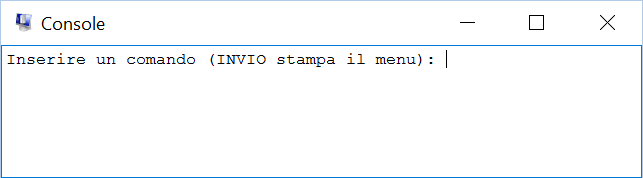
\includegraphics[scale=1]{step1.png}
       		\end{center}
       		\caption{Messaggio iniziale su consolle.}
       		\label{fig:step1}
       	\end{figure}
       	
       	\begin{figure}[h!]
       		\begin{center}
       			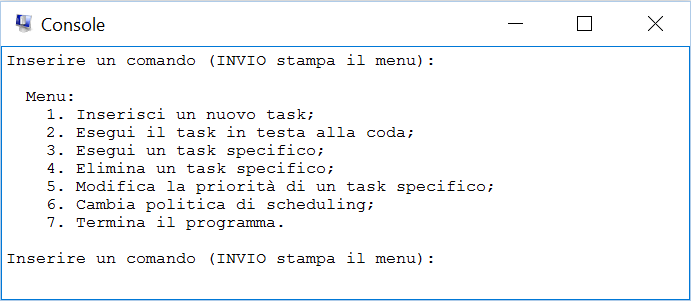
\includegraphics[scale=1]{step2.png}
       		\end{center}
       		\caption{Premendo Invio, viene stampato il menu del programma.}
       		\label{fig:step2}
       	\end{figure}
       	
       	\begin{figure}[h!]
       		\begin{center}
       			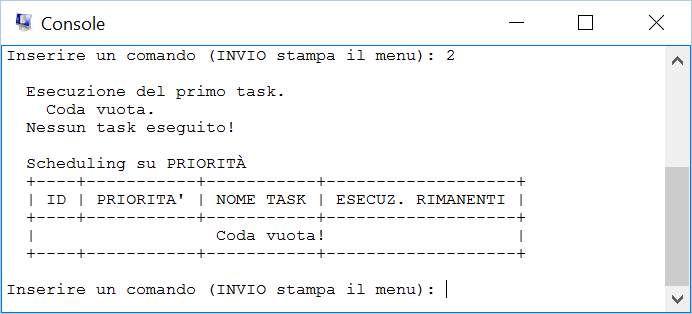
\includegraphics[scale=1]{step3.png}
       		\end{center}
       		\caption{Prima di riempire la coda, vediamo come si comportano i comandi in presenta di una coda vuota, iniziando dall'esecuzione del task in testa: nessun task viene eseguito e la tabella viene stampata.}
       		\label{fig:step3}
       	\end{figure}
       	
       	\begin{figure}[h!]
       		\begin{center}
       			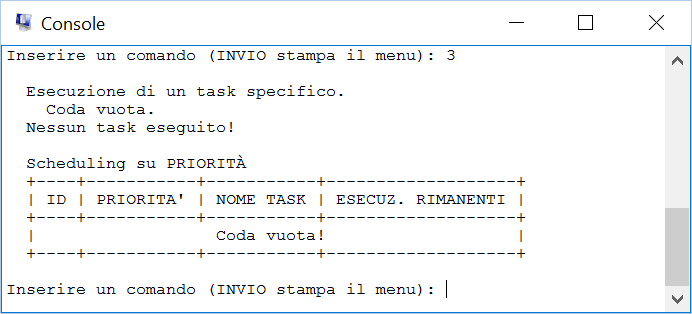
\includegraphics[scale=1]{step4.png}
       		\end{center}
       		\caption{Analogamente per l'esecuzione di un task specifico.}
       		\label{fig:step4}
       	\end{figure}
       	
       	\begin{figure}[h!]
       		\begin{center}
       			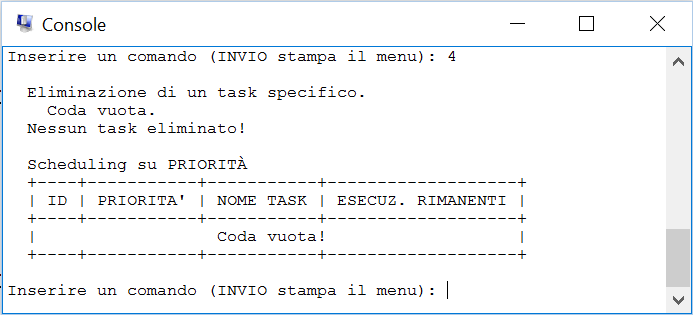
\includegraphics[scale=1]{step5.png}
       		\end{center}
       		\caption{Analogamente per l'eliminazione di un task specifico.}
       		\label{fig:step5}
       	\end{figure}
       	
       	\begin{figure}[h!]
       		\begin{center}
       			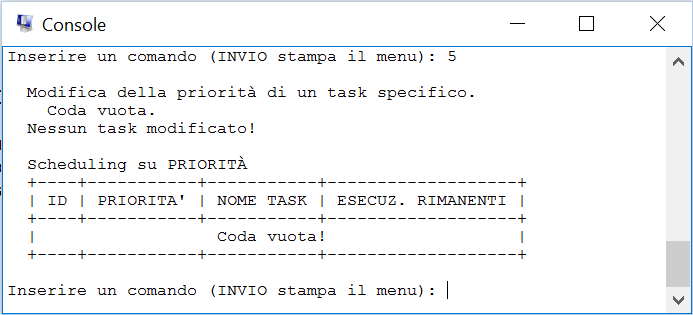
\includegraphics[scale=1]{step6.png}
       		\end{center}
       		\caption{Analogamente per la modifica della priorità di un task specifico.}
       		\label{fig:step6}
       	\end{figure}
       	
       	\begin{figure}[h!]
       		\begin{center}
       			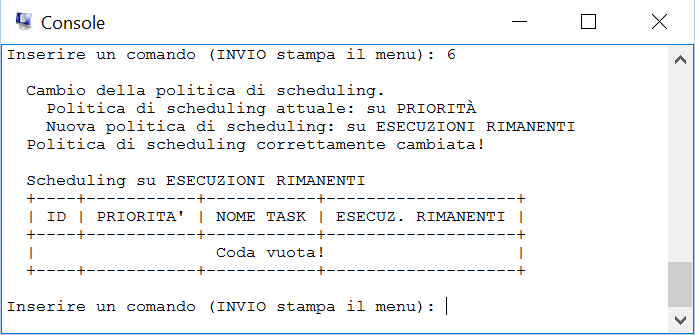
\includegraphics[scale=1]{step7.png}
       		\end{center}
       		\caption{Il cambio di politica di scheduling viene eseguito con successo e la tabella (vuota) stampata.}
       		\label{fig:step7}
       	\end{figure}
       	
       	\begin{figure}[h!]
       		\begin{center}
       			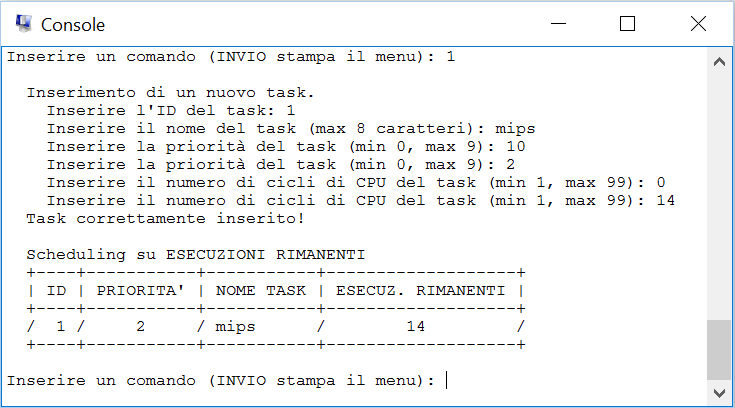
\includegraphics[scale=1]{step8.png}
       		\end{center}
       		\caption{Iniziamo ad inserire task nella coda: i dati vengono chiesti uno dopo l'altro e nel caso siano fuori dal range previsto vengono chiesti nuovamente.}
       		\label{fig:step8}
       	\end{figure}
       	
       	\begin{figure}[h!]
       		\begin{center}
       			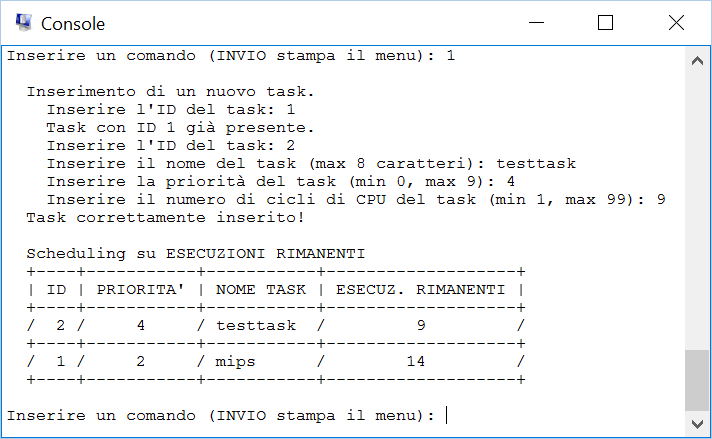
\includegraphics[scale=1]{step9.png}
       		\end{center}
       		\caption{Inseriamo un secondo elemento: vediamo che scegliere un ID già riservato comporta la richiesta di un nuovo ID.}
       		\label{fig:step9}
       	\end{figure}
       	
       	\begin{figure}[h!]
       		\begin{center}
       			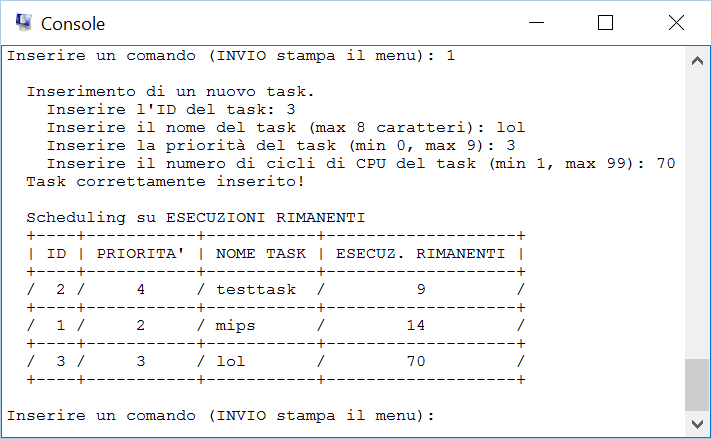
\includegraphics[scale=1]{step10.png}
       		\end{center}
       		\caption{Inseriamo un terzo elemento.}
       		\label{fig:step10}
       	\end{figure}
       	
       	\begin{figure}[h!]
       		\begin{center}
       			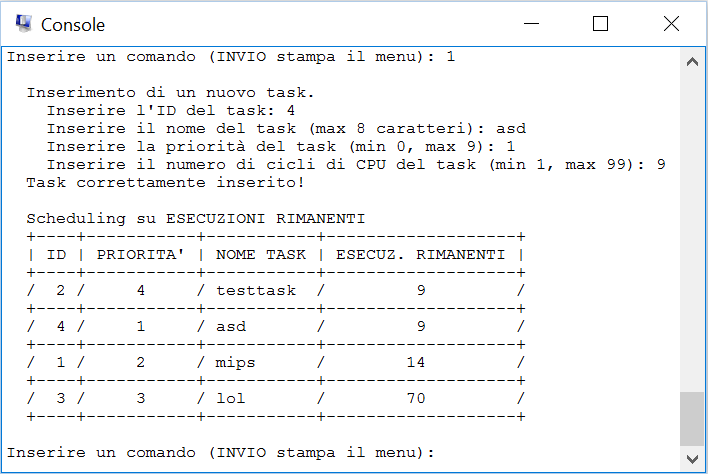
\includegraphics[scale=1]{step11.png}
       		\end{center}
       		\caption{Inseriamo un task con stesse esecuzioni rimanenti del task \textit{testtask} ma priorità minore: il nuovo task risulta correttamente più avanti nella coda.}
       		\label{fig:step11}
       	\end{figure}
       	
       	\begin{figure}[h!]
       		\begin{center}
       			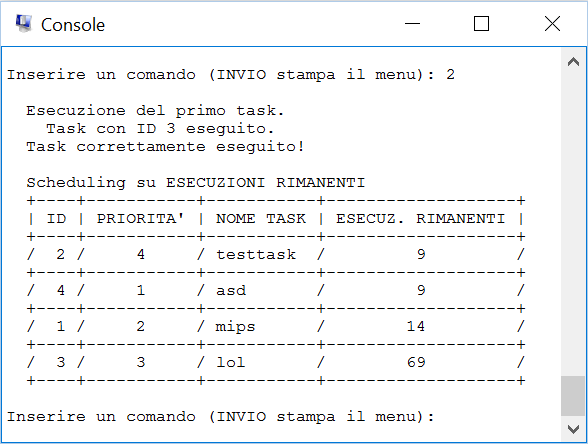
\includegraphics[scale=1]{step12.png}
       		\end{center}
       		\caption{Eseguiamo il task in testa alla coda: le esecuzioni rimanenti di \textit{lol} sono scese da $70$ a $69$.}
       		\label{fig:step12}
       	\end{figure}
       	
       	\begin{figure}[h!]
       		\begin{center}
       			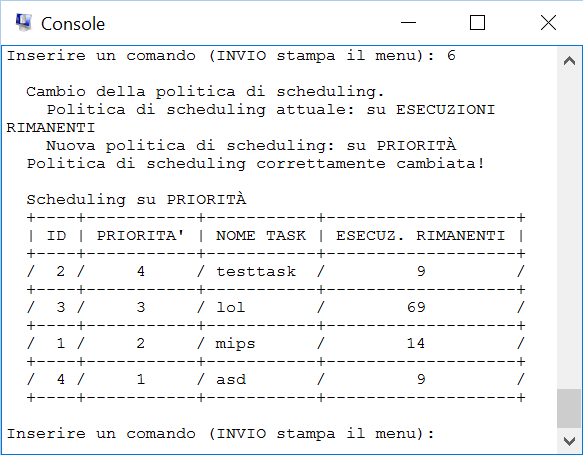
\includegraphics[scale=1]{step13.png}
       		\end{center}
       		\caption{Cambiamo la politica di scheduling di nuovo: la coda viene aggiornata di conseguenza rispettando la priorità.}
       		\label{fig:step13}
       	\end{figure}
       	
       	\begin{figure}[h!]
       		\begin{center}
       			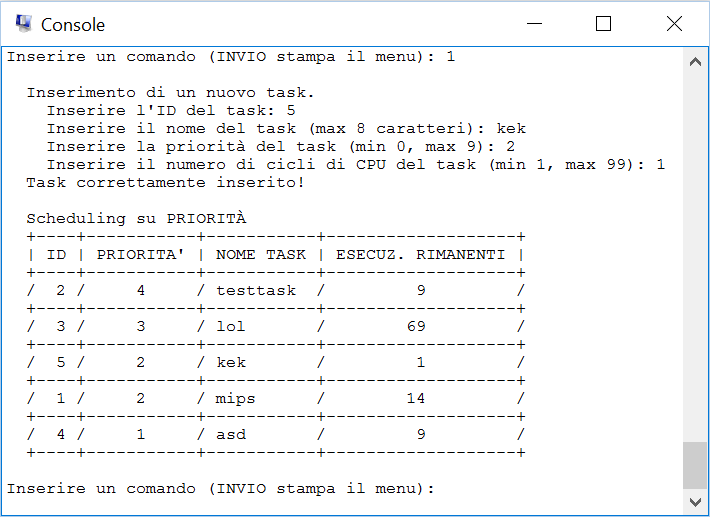
\includegraphics[scale=1]{step14.png}
       		\end{center}
       		\caption{Inseriamo un task con stessa priorità di \textit{mips} ma meno esecuzioni rimanenti: come prima, viene inserito correttamente prima di \textit{mips}.}
       		\label{fig:step14}
       	\end{figure}
       	
       	\begin{figure}[h!]
       		\begin{center}
       			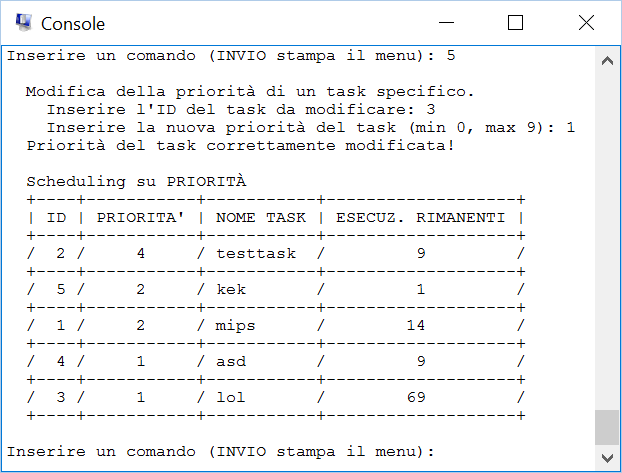
\includegraphics[scale=1]{step15.png}
       		\end{center}
       		\caption{Modifichiamo la priorità del task \textit{lol}: il task viene correttamente spostato.}
       		\label{fig:step15}
       	\end{figure}
       	
       	\begin{figure}[h!]
       		\begin{center}
       			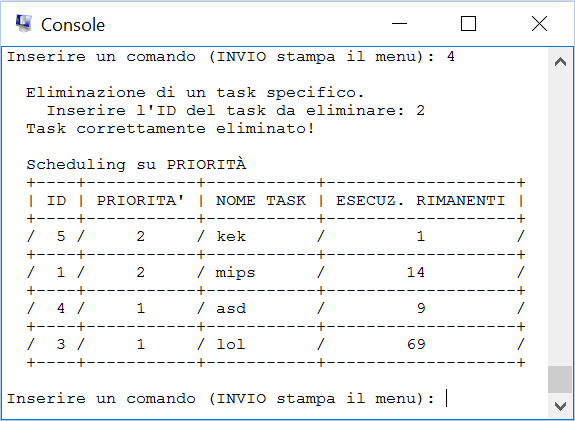
\includegraphics[scale=1]{step16.png}
       		\end{center}
       		\caption{Eliminiamo il task \textit{testtask}.}
       		\label{fig:step16}
       	\end{figure}
       	
       	\begin{figure}[h!]
       		\begin{center}
       			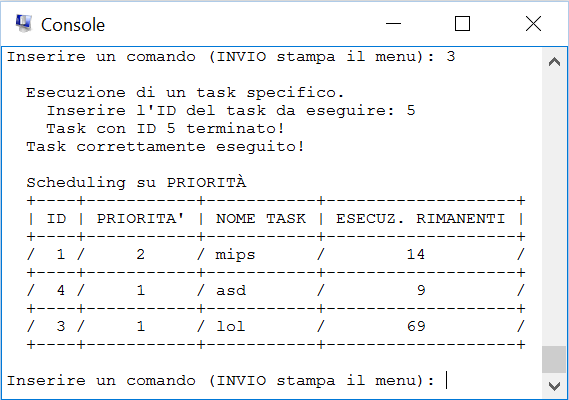
\includegraphics[scale=1]{step17.png}
       		\end{center}
       		\caption{Eseguiamo il task \textit{kek} specificandone l'ID: il task aveva $1$ esecuzione rimanente, quindi viene rimosso dalla coda.}
       		\label{fig:step17}
       	\end{figure}
       	
       	\begin{figure}[h!]
       		\begin{center}
       			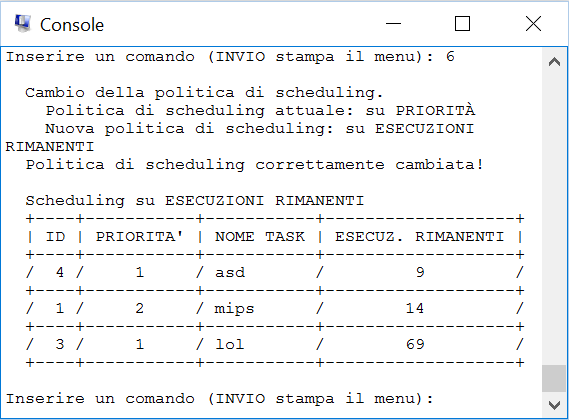
\includegraphics[scale=1]{step18.png}
       		\end{center}
       		\caption{Cambiamo politica di scheduling un'ultima volta.}
       		\label{fig:step18}
       	\end{figure}
       	
       	\begin{figure}[h!]
       		\begin{center}
       			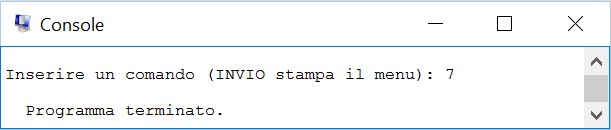
\includegraphics[scale=1]{step19.png}
       		\end{center}
       		\caption{Infine si termina il programma.}
       		\label{fig:step19}
       	\end{figure}
       	
       	\FloatBarrier
    
    \subsection*{Codice MIPS}
    
		Di seguito, il codice MIPS completo che implementa il programma descritto dal secondo esercizio, opportunamente commentato.
		
        \begin{center}
           	\begin{lstlisting}[language=mips, gobble=14, stepnumber=1]
                # Title: Scheduler di processi                  Filename: es2.s
                # Author1: ??? ?????    ???????     ???.?????@stud.unifi.it
                # Author2: ??? ?????    ???????     ???.?????@stud.unifi.it
                # Author3: ??? ?????    ???????     ???.?????@stud.unifi.it
                # Date: ??/??/????
                # Description:  Gestione dello scheduling di processi
                # Input: Comandi previsti (da 1 a 7) tramite linea di comando
                # Output: Log dell'esecuzione dei comandi scelti e coda aggiornata
                
                ################# Data segment #####################
                .data
                buffer:                     .space  1024
                tab:                        .asciiz "\t"
                newline:                    .asciiz "\n"
                insert_command:             .asciiz "Inserire un comando (INVIO stampa il menu): "
                menu:                       .asciiz "  Menu:\n    1. Inserisci un nuovo task;\n    2. Esegui il task in testa alla coda;\n    3. Esegui un task specifico;\n    4. Elimina un task specifico;\n    5. Modifica la priorità di un task specifico;\n    6. Cambia politica di scheduling;\n    7. Termina il programma.\n\n"
                exiting:                    .asciiz "  Programma terminato."
                insert_task_msg:            .asciiz "  Inserimento di un nuovo task.\n"
                insert_id_msg:              .asciiz "    Inserire l'ID del task: "
                insert_name_msg:            .asciiz "    Inserire il nome del task (max 8 caratteri): "
                insert_prio_msg:            .asciiz "    Inserire la priorità del task (min 0, max 9): "
                insert_cycles_msg:          .asciiz "    Inserire il numero di cicli di CPU del task (min 1, max 99): "
                insert_task_done_msg:       .asciiz "  Task correttamente inserito!\n\n"
                run_first_msg:              .asciiz "  Esecuzione del primo task.\n"
                empty_msg:                  .asciiz "    Coda vuota.\n"
                task_msg:                   .asciiz "    Task con ID "
                executed_msg:               .asciiz " eseguito.\n"
                completed_msg:              .asciiz " terminato!\n"
                run_done_msg:               .asciiz "  Task correttamente eseguito!\n\n"
                run_not_done_msg:           .asciiz "  Nessun task eseguito!\n\n"
                run_id_msg:                 .asciiz "  Esecuzione di un task specifico.\n"
                choose_id_msg:              .asciiz "    Inserire l'ID del task da "
                choose_id_run_msg:          .asciiz "eseguire: "
                id_not_found_msg:           .asciiz " non trovato.\n"
                id_duplicate_msg:           .asciiz " già presente.\n"
                delete_id_msg:              .asciiz "  Eliminazione di un task specifico.\n"
                choose_id_delete_msg:       .asciiz "eliminare: "
                new_prio_msg:               .asciiz "    Inserire la nuova priorità del task (min 0, max 9): "
                delete_id_done_msg:         .asciiz "  Task correttamente eliminato!\n\n"
                delete_id_not_done_msg:     .asciiz "  Nessun task eliminato!\n\n"
                change_prio_msg:            .asciiz "  Modifica della priorità di un task specifico.\n"
                choose_id_change_prio_msg:  .asciiz "modificare: "
                change_prio_done_msg:       .asciiz "  Priorità del task correttamente modificata!\n\n"
                change_prio_not_done_msg:   .asciiz "  Nessun task modificato!\n\n"
                change_sched_msg:           .asciiz "  Cambio della politica di scheduling.\n"
                change_sched_old_msg:       .asciiz "    Politica di scheduling attuale: su "
                change_sched_new_msg:       .asciiz "    Nuova politica di scheduling: su "
                change_sched_done_msg:      .asciiz "  Politica di scheduling correttamente cambiata!\n\n"
                scheduling_msg:             .asciiz "  Scheduling su "
                sched_prio_msg:             .asciiz "PRIORITÀ\n"
                sched_cycles_msg:           .asciiz "ESECUZIONI RIMANENTI\n"
                print_delim:                .asciiz "  +----+-----------+-----------+-------------------+\n"
                print_header:               .asciiz "  | ID | PRIORITA' | NOME TASK | ESECUZ. RIMANENTI |\n"
                print_empty_queue:          .asciiz "  |                  Coda vuota!                   |\n"
                print_row_start:            .asciiz "  /"
                print_row_five_spaces:      .asciiz "     "
                print_row_eight_spaces:     .asciiz "        "
                
                ################# Code segment #####################
                .text
                .globl main
                
                ### insert ###
                insert:             # procedura per l'inserimento di un task nelle liste
                    move $t0, $a0   # primo parametro: puntatore al task da inserire
                    move $t8, $a1   # secondo: puntatore alla lista A
                    move $t9, $a2   # terzo: puntatore alla lista B
                    
                    beq $t8, $zero, insert_first    # se il puntatore d'inizio è nullo (coda vuota), salta all'inserimento del primo task nella coda
                    
                    lw $t1, 20($t0) # carica la priorità
                    lw $t2, 24($t0) # e le esecuzioni rimanenti del task da inserire
                    
                    move $t3, $t8   # carica il puntatore d'inizio della lista A
                    
                insert_prio_loop:
                    lw $t4, 20($t3)                         # carica la priorità del task attuale
                    bgt $t4, $t1, insert_prio_next          # se la il task attuale ha priorità maggiore del task da inserire, passa al prossimo task
                    beq $t4, $t1, insert_prio_cycles_loop   # se la priorità è uguale, inizia a scorrere comparando le esecuzioni rimanenti
                    j insert_prio_found                     # altrimenti, si è trovato il punto in cui inserire il task
                    
                insert_prio_next:                       # istruzioni per passare al prossimo task della lista A
                    lw $t4, 28($t3)                     # carica il puntatore al prossimo task della lista A
                    beq $t4, $zero, insert_prio_last    # se il puntatore è nullo, il task è da inserire come ultimo della lista
                    move $t3, $t4                       # altrimenti, passa al prossimo
                    j insert_prio_loop                  # ed esegue un altro ciclo del loop
                    
                insert_prio_cycles_loop:                    # ciclo per la comparazione su esecuzioni rimanenti sulla lista A
                    lw $t4, 20($t3)                         # carica la priorità del task attuale
                    blt $t4, $t1, insert_prio_found         # se la priorità è minore, la sfilza di task con priorità uguale è terminata e si è trovato dove inserire il task
                    lw $t4, 24($t3)                         # altrimenti, carica le esecuzioni rimanenti del task attuale
                    blt $t4, $t2, insert_prio_cycles_next   # se le esecuzioni rimanenti del task attuale sono minori (strettamente) del task da inserire, continua a cercare comparando le esec. rimanenti
                    j insert_prio_found                     # altrimenti, si è trovato dove inserire il task
                    
                insert_prio_cycles_next:
                    lw $t4, 28($t3)                     # carica il prossimo elemento della lista A
                    beq $t4, $zero, insert_prio_last    # se il puntatore è nullo, inserisce il task come ultimo della lista
                    move $t3, $t4                       # altrimenti, passa al prossimo
                    j insert_prio_cycles_loop           # ed esegue un altro ciclo (comparando su esecuzioni rimanenti)
                    
                insert_prio_found:                      # quando il task è stato trovato
                    sw $t3, 28($t0)                     # salva il task attuale come prossimo del task da inserire
                    lw $t4, 0($t3)                      # carica il task precedente al task attuale
                    sw $t0, 0($t3)                      # imposta il task da inserire come nuovo precedente del task attuale
                    beq $t4, $zero, insert_prio_first   # se il vecchio precedente è nullo, allora il task è da inserire come primo della lista
                    sw $t4, 0($t0)                      # altrimenti, imposta il task precedente al task attuale come precedente del task da inserire
                    sw $t0, 28($t4)                     # ed imposta il task da inserire come successivo del precedente del task attuale
                    j insert_cycles                     # infine salta alle istruzioni per l'inserimento nella lista B
                    
                insert_prio_first:      # se il task è da inserire come primo della lista
                    sw $zero, 0($t0)    # salva un puntatore nullo come precedente del task da inserire
                    move $t8, $t0       # ed imposta il puntatore d'inizio della lista A al task da inserire
                    j insert_cycles     # quindi passa alla lista B
                    
                insert_prio_last:       # se il task è da inserire come ultimo della lista
                    sw $t0, 28($t3)     # salva il task da inserire come successivo del task attuale
                    sw $t3, 0($t0)      # salva il task attuale come precedente del task da inserire
                    sw $zero, 28($t0)   # ed salve un puntatore nullo come successivo del task da inserire
                    
                insert_cycles:      # le istruzioni per l'inserimento nella lista B sono speculari a quelle per la lista A
                    move $t3, $t9
                    
                insert_cycles_loop:
                    lw $t4, 24($t3)
                    blt $t4, $t2, insert_cycles_next
                    beq $t4, $t2, insert_cycles_prio_loop
                    j insert_cycles_found
                    
                insert_cycles_next:
                    lw $t4, 32($t3)
                    beq $t4, $zero, insert_cycles_last
                    move $t3, $t4
                    j insert_cycles_loop
                    
                insert_cycles_prio_loop:
                    lw $t4, 24($t3)
                    bgt $t4, $t2, insert_cycles_found
                    lw $t4, 20($t3)
                    bgt $t4, $t1, insert_cycles_prio_next
                    j insert_cycles_found
                    
                insert_cycles_prio_next:
                    lw $t4, 32($t3)
                    beq $t4, $zero, insert_cycles_last
                    move $t3, $t4
                    j insert_cycles_prio_loop
                    
                insert_cycles_found:
                    sw $t3, 32($t0)
                    lw $t4, 4($t3)
                    sw $t0, 4($t3)
                    beq $t4, $zero, insert_cycles_first
                    sw $t4, 4($t0)
                    sw $t0, 32($t4)
                    j insert_done
                    
                insert_cycles_first:
                    sw $zero, 4($t0)
                    move $t9, $t0
                    j insert_done
                    
                insert_cycles_last:
                    sw $t0, 32($t3)
                    sw $t3, 4($t0)
                    sw $zero, 32($t0)
                    j insert_done
                    
                insert_first:       # se la coda è vuota
                    move $t8, $t0   # fa puntare entrambi i puntatori d'inizio (delle due liste)
                    move $t9, $t0   # al task da inserire
                    
                insert_done:        # al termine dell'inserimento
                    move $v0, $t8   # imposta i nuovi puntatori d'inizio delle due liste
                    move $v1, $t9   # come valori di ritorno
                    jr $ra          # quindi, ritorna al chiamante
                ### insert end ###
                
                ### detach ###
                detach:             # procedura per rimuovere un task dalle liste
                    move $t0, $a0   # primo parametro: puntatore al task da rimuovere
                    move $t8, $a1   # secondo: puntatore alla lista A
                    move $t9, $a2   # terzo: puntatore alla lista B
                    
                    lw $t1, 28($t8)                     # carica il successivo del primo task nella lista A
                    beq $t1, $zero, detach_only_task    # se è nullo, allora c'è un solo task nella coda (rimuoverlo equivale a svuotare la coda)
                                                        # altrimenti
                    lw $t1, 0($t0)                      # carica il precedente del task da rimuovere
                    lw $t2, 28($t0)                     # ed il successivo
                    beq $t1, $zero, detach_first_prio   # se il puntatore al precedente è nullo, allora è da rimuovere il primo task della lista A
                    beq $t2, $zero, detach_last_prio    # se è nullo il puntatore al successivo, allora è l'ultimo
                    sw $t2, 28($t1)                     # altrimenti, imposta il successivo come successivo del precedente
                    sw $t1, 0($t2)                      # ed il precedente come precedente del successivo
                    
                    j detach_cycles # salta alla rimozione del task dalla lista B
                    
                detach_first_prio:      # se il task da rimuovere è il primo della lista A
                    move $t8, $t2       # fa puntare il puntatore d'inizio di A al task successivo (ovvero il secondo)
                    sw $zero, 0($t2)    # ed imposta il precedente del successivo come puntatore nullo
                    
                    j detach_cycles     # quindi salta alla rimozione dalla lista B
                    
                detach_last_prio:       # se il task da rimuovere è l'ultimo della lista A
                    sw $zero, 28($t1)   # basta impostare il successivo del task precedente come puntatore nullo
                    
                detach_cycles:                          # la rimozione dalla lista B è del tutto analoga a quella della lista A
                    lw $t1, 4($t0)
                    lw $t2, 32($t0)
                    beq $t1, $zero, detach_first_cycles
                    beq $t2, $zero, detach_last_cycles
                    sw $t2, 32($t1)
                    sw $t1, 4($t2)
                    
                    j detach_done
                    
                detach_first_cycles:
                    move $t9, $t2
                    sw $zero, 4($t2)
                    
                    j detach_done
                    
                detach_last_cycles:
                    sw $zero, 32($t1)
                
                    j detach_done
                    
                detach_only_task:   # se il task da rimuovere è l'unico presente nelle due code
                    move $t8, $zero # imposta i due puntatori iniziali delle liste A e B
                    move $t9, $zero # a puntatori nulli (coda vuota)
                    
                detach_done:            # una volta terminata l'eliminazione dalle due liste
                    sw $zero, 0($t0)    # imposta a puntatore nullo il precedente, nella lista A, del task rimosso
                    sw $zero, 4($t0)    # il puntatore al precedente nella lista B
                    sw $zero, 28($t0)   # il puntatore al successivo nella lista A
                    sw $zero, 32($t0)   # ed il puntatore al successivo nella lista B
                
                    move $v0, $t8       # imposta il puntatore d'inizio A come primo valore di ritorno
                    move $v1, $t9       # ed il puntatore d'inizio B come secondo valore di ritorno
                    jr $ra              # torna alla procedura chiamante
                ### detach end ###
                
                ### run ###
                run:                # procedura per l'esecuzione di un task
                    move $s0, $a0   # primo parametro: puntatore al task da eseguire
                    move $t8, $a1   # secondo: puntatore alla lista A
                    move $t9, $a2   # terzo: puntatore alla lista B
                    
                    lw $s1, 24($s0)     # carica le esecuzioni rimanenti del task
                    addi $s1, $s1, -1   # le decrementa
                    sw $s1, 24($s0)     # e salva il nuovo valore nel record del task
                    
                    addi $sp, $sp, -12  # alloca spazio nello stack per 12 byte (3 word)
                    sw $ra, 8($sp)      # salva nello stack l'indirizzo di ritorno
                    sw $s0, 4($sp)      # il puntatore al task da eseguire
                    sw $s1, 0($sp)      # ed il numero di esecuzioni rimanenti dopo la sua esecuzione
                    
                    jal detach  # chiama la funzione detach, per rimuovere il task dalle liste
                    
                    lw $t0, 4($sp)  # recupera dallo stack il puntatore al task da eseguire
                    lw $t1, 0($sp)  # e le esecuzioni rimanenti dopo l'esecuzione
                    move $t8, $v0   # come valori di ritorno di detach recupera il puntatore d'inizio A
                    move $t9, $v1   # ed il puntatore d'inizio B
                    
                    li $v0, 4           # stampa "Task con ID "
                    la $a0, task_msg
                    syscall
                    
                    li $v0, 1       # stampa l'ID del task
                    lw $a0, 8($t0)
                    syscall
                    
                    beq $t1, $zero, run_completed   # se le esecuzioni rimanenti sono zero, stampa "task terminato"
                                                    # altrimenti
                    li $v0, 4               # stampa "task eseguito"      
                    la $a0, executed_msg
                    syscall
                    
                    move $a0, $t0   # prepara il primo parametro: puntatore al task eseguito
                    move $a1, $t8   # secondo: puntatore d'inizio della lista A
                    move $a2, $t9   # terzo: puntatore d'inizio della lista B
                    
                    jal insert  # chiama la procedura insert, per reinserire il task eseguito al posto giusto
                    
                    move $t8, $v0   # recupera come valori di ritorno il puntatore d'inizio A
                    move $t9, $v1   # ed il puntatore d'inizio B
                    
                    j run_done  # salta alla fine dell'esecuzione
                    
                run_completed:              # se il task è terminato (0 esecuzioni rimanenti)
                    li $v0, 4               # stampa "task terminato"
                    la $a0, completed_msg
                    syscall
                                            # e non lo reinserisce nelle liste (eliminazione logica definitiva)
                run_done:               # al termine dell'esecuzione
                    lw $ra, 8($sp)      # recupera l'indirizzo di ritorno dallo stack
                    addi $sp, $sp, 12   # dealloca lo stack frame
                    
                    move $v0, $t8   # imposta come valori di ritorno il puntatore d'inizio A
                    move $v1, $t9   # ed il puntatore d'inizio B
                    jr $ra          # torna al chiamante
                ### run end ###
                
                ### find_id ###
                find_id:            # procedura per recuperare un task con un ID specifico
                    move $t0, $a0   # primo argomento: ID del task da recuperare
                    move $t8, $a1   # secondo: puntatore d'inizio della lista A
                    
                    move $t1, $zero # puntatore al task con ID cercato, inizializzato come nullo
                    
                find_id_loop:
                    lw $t2, 8($t8)              # carica l'ID del task attuale
                    beq $t2, $t0, find_id_found # se gli ID coincidono, allora il task è stato trovato
                    lw $t2, 28($t8)             # altrimenti, carica il puntatore al task successivo
                    beq $t2, $zero, find_id_end # se è nullo, allora si è raggiunta la fine senza trovare il task
                    move $t8, $t2               # altrimenti passa al successivo
                    j find_id_loop              # ed esegue un altro ciclo
                    
                find_id_found:      # se il task è stato trovato
                    move $t1, $t8   # salva il puntatore al task
                    
                find_id_end:        # alla fine della procedura
                    move $v0, $t1   # restituisce il puntatore al task trovato, o null se non è stato trovato
                    jr $ra          # torna al chiamante
                ### find_id end ###
                
                ### insert_task ###
                insert_task:		# procedura per l'inserimento di un nuovo task
                					# primo argomento: ignorato
                    move $s6, $a1	# secondo: puntatore d'inizio A
                    move $s7, $a2	# terzo: puntatore d'inizio B
                    
                    addi $sp, $sp, -20	# alloca 20 byte (5 word) nello stack frame
                    sw $ra, 16($sp)		# salva nello stack: il puntatore di ritorno al chiamante
                    sw $s6, 12($sp)		# il puntatore d'inizio della lista A
                    sw $s7, 8($sp)		# ed il puntatore d'inizio della lista B
                
                    li $v0, 4               # stampa la stringa d'inizio dell'inserimento di un task
                    la $a0, insert_task_msg
                    syscall
                    
                    li $v0, 9   # chiamata sbrk
                    li $a0, 36  # 36 byte totali (9 word)
                    syscall     # puntatore al precedente A (4 byte, 0-4)
                                # puntatore al precedente B (4 byte, 4-8)
                                # ID (4 byte, 8-12)
                                # nome (8 byte, 12-20)
                                # priorità (4 byte, 20-24)
                                # esecuzioni rimanenti (4 byte, 24-28)
                                # puntatore al successivo A (4 byte, 28-32)
                                # puntatore al successivo B (4 byte, 32-36)
                                
                    move $s0, $v0   # salva l'indirizzo d'inizio dei 36 byte allocati in $s0
                    sw $s0, 4($sp)	# e lo salva nello stack
                    
                    sw $zero, 0($s0)    # salva nell'heap: il puntatore al precedente A
                    sw $zero, 4($s0)    # e il puntatore al precedente B
                    
                insert_task_id:
                    li $v0, 4				# chiede di inserire l'ID del task
                    la $a0, insert_id_msg
                    syscall
                    
                    li $v0, 5		# legge un intero da input
                    syscall
                    move $s1, $v0
                    
                    beq $s6, $zero, insert_task_id_store	# se la coda è vuota, salva l'ID inserito
                											# altrimenti
                    sw $s1, 0($sp)	# salva l'ID inserito nello stack
                    
                    move $a0, $s1	# prepare il primo argomento: ID inserito
                    move $a1, $s6	# secondo argomento: puntatore d'inizio A
                    
                    jal find_id	# invoca la procedura find_id
                    
                    move $t1, $v0	# salva in $t1 il risultato di find_id
                    lw $s6, 12($sp)	# recupera dallo stack: il puntatore d'inizio A
                    lw $s7, 8($sp)	# il puntatore d'inizio B
                    lw $s0, 4($sp)	# il puntatore alrecord allocato nell'heap
                    lw $t0, 0($sp)	# ed il valore dell'ID inserito
                    
                    bne $t1, $zero, insert_task_id_duplicate	# se il puntatore ritornato da find_id è non nullo, esiste già un task con l'ID inserito
                    j insert_task_id_store						# altrimenti, può memorizzare l'ID tranquillamente
                    
                insert_task_id_duplicate:	# se è già presente in coda un task con l'ID inserito
                    li $v0, 4			#  stampa un messaggio d'errore
                    la $a0, task_msg
                    syscall
                    
                    li $v0, 1
                    move $a0, $t0
                    syscall
                    
                    li $v0, 4
                    la $a0, id_duplicate_msg
                    syscall
                    
                    j insert_task_id	# torna nuovamente all'inserimento dell'ID
                    
                insert_task_id_store:	# se non si sono trovati ID duplicati
                    sw $t0, 8($s0)	# memorizza l'ID nell'heap
                    
                insert_task_name:
                    li $v0, 4				# chiede di inserire il nome del task
                    la $a0, insert_name_msg
                    syscall
                    
                    li $v0, 8		# legge una stringa
                    la $a0, buffer
                    li $a1, 1024
                    syscall
                    
                    li $t0, 0	# contatore inizializzato a zero (caratteri copiati nell'heap)
                    
                insert_task_name_loop:
                    li $t1, 8						# carica l'intero 8
                    beq $t0, $t1, insert_task_prio	# se il contatore ha raggiunto 8, salta all'inserimento della priorità
                									# altrimenti
                    la $t1, buffer		# carica l'indirizzo di base della stringa inserita
                    add $t1, $t1, $t0	# shhifta l'indirizzo in avanti del numero di caratteri già copiati (diciamo n)
                    lb $t2, 0($t1)		# carica il carattere n-esimo della stringa
                	
                    li $t3, 32								# carica l'intero 32 (primo carattere non speciale nella codifica ASCII)
                    blt $t2, $t3, insert_task_name_spaces	# se il carattere letto è un carattere speciale, inizia il loop per inserire spazi
                											# altrimenti	
                    addi $t1, $s0, 12	# carica l'indirizzo base del campo nome del task (indirizzo base del record + 12 byte)
                    add $t1, $t1, $t0	# ci somma il numero di caratteri letti (prima posizione del nome non copiata)
                    sb $t2, 0($t1)		# copia il carattere nell'heap
                	
                    addi $t0, $t0, 1		# incrementa il contatore
                    j insert_task_name_loop	# esegue un altro ciclo
                    
                insert_task_name_spaces:			# se si è trovato un carattere speciale
                    li $t1, 8						# se si sono copiati 8 caratteri
                    beq $t0, $t1, insert_task_prio	# finisce il ciclo
                									# altrimenti
                    addi $t1, $s0, 12	# carica l'indirizzo della prima posizione del nome disponibile
                    add $t1, $t1, $t0
                    li $t2, ' '			# e ci copia uno spazio
                    sb $t2, 0($t1)
                	
                    addi $t0, $t0, 1			# incrementa il contatore
                    j insert_task_name_spaces	# ed esegue un altro ciclo
                    
                insert_task_prio:
                    li $v0, 4				# chiede di inserire la priorità del task
                    la $a0, insert_prio_msg
                    syscall
                    
                    li $v0, 5	# legge  un intero da input
                    syscall
                    
                    li $t0, 0                           # se si è inserita una priorità minore di 0
                    blt $v0, $t0, insert_task_prio
                    li $t0, 9                           # o se si è inserita una priorità maggiore di 9
                    bgt $v0, $t0, insert_task_prio      # chiede nuovamente la priorità del task
                    sw $v0, 20($s0)                     # altrimenti salva nell'heap
                    
                insert_task_cycles:
                    li $v0, 4					# chiede di inserire i cicli di esecuzione totali del task
                    la $a0, insert_cycles_msg
                    syscall
                    
                    li $v0, 5	# legge un intero da input
                    syscall
                    
                    li $t0, 1                           # se si sono inseriti meno di 1 ciclo
                    blt $v0, $t0, insert_task_cycles
                    li $t0, 99                          # o se si sono inseriti più di 99 cicli
                    bgt $v0, $t0, insert_task_cycles    # chiede nuovamente i cicli del task
                    sw $v0, 24($s0)                     # altrimenti salva nell'heap
                    
                    sw $zero, 28($s0)	# salva nell'heap: il puntatore al successivo A
                    sw $zero, 32($s0)	# ed il puntatore al successivo B
                    
                    move $a0, $s0	# prepara il primo argomento: puntatore al task appena creato (da inserire)
                    move $a1, $s6	# secondo: puntatore d'inizio A
                    move $a2, $s7	# terzo: puntatore d'inizio B
                    
                    jal insert	# invoca la procedura insert
                    
                    move $s6, $v0	# recupera i valori di ritorno di insert: puntatore d'inizio A
                    move $s7, $v1	# puntatore d'inizio B
                
                    li $v0, 4						# stampa il corretto inserimento del task
                    la $a0, insert_task_done_msg
                    syscall
                    
                    lw $ra, 16($sp)		# recupera l'indirizzo di ritorno al chiamante
                    addi $sp, $sp, 20	# dealloca lo stack
                    
                    move $v0, $s6	# prepara i valori di ritorno: puntatore alla lista A
                    move $v1, $s7	# puntatore alla lista B
                    
                    jr $ra	# torna al chiamante
                ### insert_task end ###
                
                ### run_first ###
                run_first:			# procedura per eseguire il task in testa alla coda
                    move $t7, $a0	# primo argomento: politica di scheduling
                    move $t8, $a1	# secondo: puntatore d'inizio A
                    move $t9, $a2	# terzo: puntatore d'inizio B
                
                    li $v0, 4               # stampa la stringa d'inizio dell'esecuzione del primo task
                    la $a0, run_first_msg
                    syscall
                    
                    li $t0, 'a'						# carica il carattere 'a'
                    bne $t7, $t0, run_first_cycles	# se la politica di scheduling non è A,  passa all'inizializzazione per la politica B
                    move $t1, $t8					# altrimenti, carica il puntatore d'inizio di A
                    
                    j run_first_check_empty	# controlla se la coda è vuota
                    
                run_first_cycles:	# se la politica è B
                    move $t1, $t9	# carica il puntatore d'inizio B
                    
                run_first_check_empty:				# controlla se la coda è vuota
                    beq $t1, $zero, run_first_empty	# se il puntatore d'inizio è nullo, la coda è vuota
                									# altrimenti
                run_first_loop:
                    bne $t7, $t0, run_first_load_next_cycles	# se la politica non è A, carica il seguente della lista B
                												# altrimenti
                    lw $t2, 28($t1)			# carica il seguente della lista A
                    j run_first_check_next	# salta al controllo dell'elemento successivo
                    
                run_first_load_next_cycles:	# se la politica non era A
                    lw $t2, 32($t1)			# carica il successivo della lista B
                    
                run_first_check_next:				# controllo dell'elemento successivo
                    beq $t2, $zero, run_first_found	# se il puntatore all'elemento seguente è nullo, allora il task in testa è stato trovato
                									# altrimenti
                    move $t1, $t2		# passa al seguente
                    j run_first_loop	# ed esegue un altro ciclo
                
                run_first_found:		# quando l'elemento in testa è trovato
                    addi $sp, $sp, -4	# alloca 4 byte nello stack frame (1 word)
                    sw $ra, 0($sp)		# salva l'indirizzo di ritorno nello stack
                    
                    move $a0, $t1	# prepara il primo parametro: puntatore al task in testa alla coda
                    move $a1, $t8	# secondo: puntatore d'inizio A
                    move $a2, $t9	# terzo: puntatore d'inizio B
                    
                    jal run	# invoca la procedura run
                    
                    move $t8, $v0	# recupera i valori di ritorno di run: puntatore d'inizio A
                    move $t9, $v1	# e puntatore d'inizio B
                    
                    lw $ra, 0($sp)		# recupera l'indirizzo di ritorno al chiamante dallo stack
                    addi $sp, $sp, 4	# e dealloca lo stack frame
                
                    j run_first_done	# salta alla terminazione (con successo) della proocedura run_first
                        
                run_first_empty:		# se la coda era vuota
                    li $v0, 4			# stampa un messaggio indicando l'errore
                    la $a0, empty_msg
                    syscall
                    
                    li $v0, 4
                    la $a0, run_not_done_msg
                    syscall
                    
                    j run_first_return	# salta alle istruzioni di ritorno
                
                run_first_done:				# se la procedura è terminata con successo
                    li $v0, 4				# stampa un messagggio di terminazione
                    la $a0, run_done_msg
                    syscall
                    
                run_first_return:
                    move $v0, $t8	# prepara i valori di ritorno: puntatore d'inizio A
                    move $v1, $t9	# e puntatore d'inizio B
                
                    jr $ra	# torna al chiamante
                ### run_first end ###
                
                ### run_id ###
                run_id:					# procedura per eseguire un task specifico
                    addi $sp, $sp, -16	# alloca 16 byte nello stack frame (4 word)
                    sw $ra, 12($sp)		# salva l'indirizzo di ritorno nello stack
                
                					# primo argomento: ignorato
                    move $s6, $a1	# secondo: puntatore d'inizio A
                    move $s7, $a2	# terzo: puntatore d'inizio B
                    
                    sw $s6, 8($sp)	# salva nello stack: il puntatore d'inizio A
                    sw $s7, 4($sp)	# ed il puntatore d'inizio B
                
                    li $v0, 4               # stampa la stringa d'inizio dell'esecuzione di un task specifico
                    la $a0, run_id_msg
                    syscall
                    
                    beq $s6, $zero, run_id_empty	# se il puntatore d'inizio è nullo, allora la coda è vuota
                    
                run_id_choose:
                    li $v0, 4				# chiede di inserire l'ID del task da eseguire
                    la $a0, choose_id_msg
                    syscall
                    
                    li $v0, 4
                    la $a0, choose_id_run_msg
                    syscall
                    
                    li $v0, 5		# legge un intero da input
                    syscall
                    move $s0, $v0	# lo salva in $s0
                    sw $s0, 0($sp)	# e lo salva nello stack
                    
                    move $a0, $s0	# prepara il primo parametro d'invocazione: ID inserito
                    move $a1, $s6	# secondo: puntatore d'inizio A
                    
                    jal find_id	# invoca la procedura find_id
                    
                    move $t0, $v0	# recupera il valore di ritorno di find_id
                    lw $s6, 8($sp)	# recupera dallo stack: il puntatore d'inizio A
                    lw $s7, 4($sp)	# ed il puntatore d'inizio B
                    
                    beq $t0, $zero, run_id_not_found	# se il puntatore restituito da find_id è nullo, allora non c'è nessun task con l'ID inserito
                										# altrimenti
                    move $a0, $t0	# prepara il primo parametro: puntatore al task con ID selezionato
                    move $a1, $s6	# secondo: puntatore d'inizio A
                    move $a2, $s7	# terzo: puntatore d'inizio B
                    
                    jal run	# invoca la procedura run
                    
                    move $s6, $v0   # recupera i valori di ritorno: puntatore d'inizio A
                    move $s7, $v1   # e puntatore d'inizio B
                    
                    j run_id_done   # salta alla terminazione con successo della procedura
                
                run_id_not_found:       # se il task con ID selezionato non è stato trovato
                    li $v0, 4           # stampa un messaggio d'errore
                    la $a0, task_msg
                    syscall
                    
                    li $v0, 1
                    lw $a0, 0($sp)
                    syscall
                    
                    li $v0, 4
                    la $a0, id_not_found_msg
                    syscall
                    
                    j run_id_choose # e torna all'inserimento dell'ID
                    
                run_id_empty:           # se la coda era vuota
                    li $v0, 4           # stampa un messaggio d'errore
                    la $a0, empty_msg
                    syscall
                    
                    li $v0, 4
                    la $a0, run_not_done_msg
                    syscall
                    
                    j run_id_return # e ritorna
                    
                run_id_done:                # se l'esecuzione è eseguita con successo
                    li $v0, 4               # stampa un messaggio di corretta terminazione
                    la $a0, run_done_msg
                    syscall
                
                run_id_return:
                    move $v0, $s6   # prepara i valori di ritorno: puntatore d'inizio A
                    move $v1, $s7   # e puntatore d'inizio B
                    
                    lw $ra, 12($sp)     # recupera l'indirizzo di ritorno dallo stack
                    addi $sp, $sp, 16   # e dealloca lo stack frame
                    
                    jr $ra  # torna al chiamante
                ### run_id end ###
                
                ### delete_id ###
                delete_id:              # analogo a run_id, cambia soltanto la parte centrale
                    addi $sp, $sp, -16
                    sw $ra, 12($sp)
                
                    move $s6, $a1
                    move $s7, $a2
                    
                    sw $s6, 8($sp)
                    sw $s7, 4($sp)
                
                    li $v0, 4
                    la $a0, delete_id_msg
                    syscall
                    
                    beq $s6, $zero, delete_id_empty
                    
                delete_id_choose:
                    li $v0, 4
                    la $a0, choose_id_msg
                    syscall
                    
                    li $v0, 4
                    la $a0, choose_id_delete_msg
                    syscall
                    
                    li $v0, 5
                    syscall
                    move $s0, $v0
                    sw $s0, 0($sp)
                    
                    move $a0, $s0
                    move $a1, $s6
                    
                    jal find_id
                    
                    move $t0, $v0
                    lw $s6, 8($sp)
                    lw $s7, 4($sp)
                    
                    beq $t0, $zero, delete_id_not_found
                
                    move $a0, $t0
                    move $a1, $s6
                    move $a2, $s7
                    
                    jal detach  # invoca la procedura detach
                    
                    move $s6, $v0
                    move $s7, $v1
                    
                    j delete_id_done
                
                delete_id_not_found:
                    li $v0, 4
                    la $a0, task_msg
                    syscall
                    
                    li $v0, 1
                    lw $a0, 0($sp)
                    syscall
                    
                    li $v0, 4
                    la $a0, id_not_found_msg
                    syscall
                    
                    j delete_id_choose
                    
                delete_id_empty:
                    li $v0, 4
                    la $a0, empty_msg
                    syscall
                    
                    li $v0, 4
                    la $a0, delete_id_not_done_msg
                    syscall
                    
                    j delete_id_return
                    
                delete_id_done:
                    li $v0, 4
                    la $a0, delete_id_done_msg
                    syscall
                
                delete_id_return:
                    move $v0, $t8
                    move $v1, $t9
                    
                    lw $ra, 12($sp)
                    addi $sp, $sp, 16
                    
                    jr $ra
                ### delete_id end ###
                    
                ### change_prio ###
                change_prio:            # analogo a run_id, cambia soltanto la parte centrale
                    addi $sp, $sp, -20
                    sw $ra, 16($sp)
                
                    move $s6, $a1
                    move $s7, $a2
                    
                    sw $s6, 12($sp)
                    sw $s7, 8($sp)
                
                    li $v0, 4
                    la $a0, change_prio_msg
                    syscall
                    
                    beq $s6, $zero, change_prio_empty
                    
                change_prio_choose:
                    li $v0, 4
                    la $a0, choose_id_msg
                    syscall
                    
                    li $v0, 4
                    la $a0, choose_id_change_prio_msg
                    syscall
                    
                    li $v0, 5
                    syscall
                    move $s0, $v0
                    sw $s0, 4($sp)
                    
                    move $a0, $s0
                    move $a1, $s6
                    
                    jal find_id
                    
                    move $s1, $v0
                    sw $s1, 0($sp)
                    lw $s6, 12($sp)
                    lw $s7, 8($sp)
                    
                    beq $s1, $zero, change_prio_not_found
                    
                change_prio_insert_new:
                    li $v0, 4               # chiede la nuova priorità del task
                    la $a0, new_prio_msg
                    syscall
                    
                    li $v0, 5       # legge un intero
                    syscall
                    move $t0, $v0   # e lo salva in $t0
                
                    li $t1, 0                               # se si è inserita una priorità minore di 0
                    blt $t0, $t1, change_prio_insert_new
                    li $t1, 9                               # o se si è inserita una priorità maggiore di 9
                    bgt $t0, $t1, change_prio_insert_new    # chiedi nuovamente la priorità del task
                    sw $t0, 20($s1)                         # altrimenti aggiorna la priorità nell'heap
                
                    move $a0, $s1   # prepara il primo parametro: puntatore al task da modificare
                    move $a1, $s6   # secondo: puntatore d'inizio A
                    move $a2, $s7   # terzo: puntatore d'inizio B
                    
                    jal detach  # invoca la procedura detach
                    
                    lw $s1, 0($sp)  # recupera il puntatore al task da modificare dallo stack
                    move $s6, $v0   # recupera i valori di ritorno: puntatore d'inizio A
                    move $s7, $v1   # e puntatore d'inizio B
                    
                    move $a0, $s1   # prepara i parametri (come prima)
                    move $a1, $s6
                    move $a2, $s7
                    
                    jal insert  # invoca la procedura insert
                    
                    move $s6, $v0   # recupera i valori di ritorno (come prima)
                    move $s7, $v1
                    
                    j change_prio_done
                
                change_prio_not_found:
                    li $v0, 4
                    la $a0, task_msg
                    syscall
                    
                    li $v0, 1
                    lw $a0, 4($sp)
                    syscall
                    
                    li $v0, 4
                    la $a0, id_not_found_msg
                    syscall
                    
                    j change_prio_choose
                    
                change_prio_empty:
                    li $v0, 4
                    la $a0, empty_msg
                    syscall
                    
                    li $v0, 4
                    la $a0, change_prio_not_done_msg
                    syscall
                    
                    j change_prio_return
                    
                change_prio_done:
                    li $v0, 4
                    la $a0, change_prio_done_msg
                    syscall
                
                change_prio_return:
                    move $v0, $s6
                    move $v1, $s7
                    
                    lw $ra, 16($sp)
                    addi $sp, $sp, 20
                    
                    jr $ra
                ### change_prio end ###
                
                ### change_sched ###
                change_sched:   # procedura per cambiare la politica di scheduling
                    move $t7, $a0   # primo parametro: politica di scheduling attuale
                                    # secondo e terzo parametro: ignorati
                    
                    li $v0, 4                   # stampa la stringa d'inizio del cambio della politica di scheduling
                    la $a0, change_sched_msg
                    syscall
                    
                    li $v0, 4                       # stampa "Politica di scheduling attuale:"
                    la $a0, change_sched_old_msg
                    syscall
                    
                    li $t0, 'a'                         # carica il carattere 'a'
                    bne $t7, $t0, change_sched_to_prio  # se la politica di scheduling attuale non è A, viene cambiata ad A
                                                        # altrimenti
                    li $v0, 4               # stampa la politica attuale (su PRIORITÀ)
                    la $a0, sched_prio_msg
                    syscall
                    
                    li $t7, 'b' # cambia la politica a B
                    
                    li $v0, 4                       # stampa la nuova politica (su ESECUZIONI RIMANENTI)
                    la $a0, change_sched_new_msg
                    syscall
                    
                    li $v0, 4
                    la $a0, sched_cycles_msg
                    syscall
                    
                    j change_sched_end  # salta alla fine della procedura
                    
                change_sched_to_prio:           # se la politica non era A
                    li $v0, 4                   # stampa la politica attuale (su ESECUZIONI RIMANENTI)
                    la $a0, sched_cycles_msg
                    syscall
                
                    li $t7, 'a' # cambia la politica ad A
                    
                    li $v0, 4                       # stampa la nuova politica (su PRIORITA)
                    la $a0, change_sched_new_msg
                    syscall
                    
                    li $v0, 4
                    la $a0, sched_prio_msg
                    syscall
                    
                change_sched_end:
                    li $v0, 4                       # stampa un messaggio di corretta terminazione della procedura
                    la $a0, change_sched_done_msg
                    syscall
                    
                    move $v0, $t7   # imposta la nuova politica di scheduling come valore di ritorno
                    
                    jr $ra  # ritorna al chiamante
                ### change_sched end ###
                
                ### Main ###
                main:
                    li $s5, 'a'     # inizializza la politica di scheduling ad A (scheduling su priorità)
                    move $s6, $zero # ed il puntatore alla coda A
                    move $s7, $zero # e alla coda B a 0 (nessun elemento in coda)
                
                command_selection:
                    li $v0, 4               # stampa la stringa per la selezione del comando
                    la $a0, insert_command
                    syscall
                    
                    li $v0, 5       # legge un intero in input
                    syscall
                    move $t0, $v0   # salva l'intero letto in $t0
                    
                    li $v0, 4       # stampa una newline
                    la $a0, newline
                    syscall
                    
                    move $a0, $s5   # prepara il primo parametro (politica di scheduling)
                    move $a1, $s6   # il secondo (puntatore ad A)
                    move $a2, $s7   # ed il terzo (puntatore a B)
                    
                    li $t1, 1                       # se l'intero letto è 1
                    beq $t0, $t1, jump_insert_task  # il comando da eseguire è l'inserimento di un nuovo task
                    li $t1, 2                       # se è 2
                    beq $t0, $t1, jump_run_first    # il comando da eseguire è l'esecuzione del primo task
                    li $t1, 3                       # se è 3
                    beq $t0, $t1, jump_run_id       # il comando da eseguire è l'esecuzione di un task specifico
                    li $t1, 4                       # se è 4
                    beq $t0, $t1, jump_delete_id    # il comando da eseguire è l'eminazione di un task specifico
                    li $t1, 5                       # se è 5
                    beq $t0, $t1, jump_change_prio  # il comando da eseguire è la modifica della priorità di un task specifico
                    li $t1, 6                       # se è 6
                    beq $t0, $t1, jump_change_sched # il comando da eseguire è il cambio della politica di scheduling
                    li $t1, 7                       # se è 7
                    beq $t0, $t1, exit              # il comando da eseguire è la terminazione del programma
                                    #altrimenti
                    li $v0, 4       # stampa il menu
                    la $a0, menu
                    syscall
                    
                    j command_selection # e torna alla selezione del comando
                    
                jump_insert_task:       # prepara il necessario per il salto al comando d'inserimento
                    addi $sp, $sp, -4   # alloca 4 byte nello stack frame
                    sb $s5, 0($sp)      # salva la politica di scheduling nello stack
                    
                    jal insert_task # salta alla procedura per l'inserimento di un task
                                    # recupera i risultati della procedura
                    move $s6, $v0   # ovvero il puntatore ad A
                    move $s7, $v1   # ed il puntatore a B
                    
                    lb $s5, 0($sp)      # recupera la politica di scheduling dallo stack
                    addi $sp, $sp, 4    # dealloca i 4 byte dallo stack
                    
                    j print_queue   # salta alle istruzioni per la stampa della coda
                    
                jump_run_first:         # jump_run_first, jump_run_id, jump_delete_id e jump_change_prio analoghi a jump_insert_task
                    addi $sp, $sp, -4
                    sb $s5, 0($sp)
                    
                    jal run_first
                    
                    move $s6, $v0
                    move $s7, $v1
                    
                    lb $s5, 0($sp)
                    addi $sp, $sp, 4
                    
                    j print_queue
                    
                jump_run_id:
                    addi $sp, $sp, -4
                    sb $s5, 0($sp)
                    
                    jal run_id
                    
                    move $s6, $v0
                    move $s7, $v1
                    
                    lb $s5, 0($sp)
                    addi $sp, $sp, 4
                    
                    j print_queue
                    
                jump_delete_id:
                    addi $sp, $sp, -4
                    sb $s5, 0($sp)
                    
                    jal delete_id
                    
                    move $s6, $v0
                    move $s7, $v1
                    
                    lb $s5, 0($sp)
                    addi $sp, $sp, 4
                    
                    j print_queue
                    
                jump_change_prio:
                    addi $sp, $sp, -4
                    sb $s5, 0($sp)
                    
                    jal change_prio
                    
                    move $s6, $v0
                    move $s7, $v1
                    
                    lb $s5, 0($sp)
                    addi $sp, $sp, 4
                    
                    j print_queue
                    
                jump_change_sched:      # analogo agli altri jump
                    addi $sp, $sp, -8   # con la differenza che nello stack si salvano i due puntatori
                    sw $s6, 4($sp)      # e la procedura ritorna la nuova politica di scheduling
                    sw $s7, 0($sp)
                    
                    jal change_sched
                    
                    move $s5, $v0
                    
                    lw $s6, 4($sp)
                    lw $s7, 0($sp)
                    addi $sp, $sp, 8
                    
                    j print_queue
                    
                print_queue:                # istruzioni per la stampa della coda
                    li $v0, 4               # stampa "Scheduling su"
                    la $a0, scheduling_msg  # il nome effettivo viene poi stampato a seconda dello scheduling attuale
                    syscall
                
                    li $t0, 'a'                             # carica il carattere 'a', per poterlo comparare con la politica attuale
                    bne $s5, $t0, print_queue_cycles_begin  # se la politica non è A, esegui l'inizializzazione per la politica B
                                                            # altrimenti
                    move $t1, $s6   # inizializza il puntatore $t1 col puntatore di A
                    
                    li $v0, 4               # stampa "PRIORITÀ"
                    la $a0, sched_prio_msg
                    syscall
                    
                    j print_queue_header    # salta alla stampa dell'header della tabella
                    
                print_queue_cycles_begin:   # se la politica è B
                    move $t1, $s7           # inizializza il puntatore $t1 col puntatore di B
                
                    li $v0, 4                   # stampa "ESECUZIONI RIMANENTI"
                    la $a0, sched_cycles_msg
                    syscall
                    
                print_queue_header:
                    
                    li $v0, 4           # stampa un delimitatore
                    la $a0, print_delim
                    syscall
                    
                    li $v0, 4               # stampa l'header
                    la $a0, print_header
                    syscall
                    
                    li $v0, 4           # stampa un delimitatore
                    la $a0, print_delim
                    syscall
                    
                    beq $t1, $zero, print_queue_empty   # se il puntatore d'inizio è zero, salta alla stampa della coda vuota
                    
                print_queue_loop:
                    li $v0, 4               # stampa l'inizio di una riga
                    la $a0, print_row_start
                    syscall
                    
                    lw $t2, 8($t1)                  # carica l'ID del task attuale
                    li $t3, 9                       # se è composto da due cifre
                    bgt $t2, $t3, print_queue_id    # stampa subito l'ID
                                                    # altrimenti
                    li $v0, 11  # stampa prima uno spazio extra
                    li $a0, ' '
                    syscall
                    
                print_queue_id:
                    li $v0, 11  # stampa uno spazio
                    li $a0, ' '
                    syscall
                
                    li $v0, 1       # stampa l'ID
                    move $a0, $t2
                    syscall
                    
                    li $v0, 11  # stampa uno spazio
                    li $a0, ' '
                    syscall
                    
                    li $v0, 11  # ed un separatore
                    li $a0, '/'
                    syscall
                    
                    li $v0, 4                       # stampa cinque spazi
                    la $a0, print_row_five_spaces
                    syscall
                    
                    li $v0, 1       # stampa la priorità
                    lw $a0, 20($t1)
                    syscall
                    
                    li $v0, 4                       # stampa altri cinque spazi
                    la $a0, print_row_five_spaces
                    syscall
                    
                    li $v0, 11  # stampa un separatore
                    li $a0, '/'
                    syscall
                    
                    li $v0, 11  # ed uno spazio
                    li $a0, ' '
                    syscall
                    
                    li $t2, 12  # carica 12 (offset d'inizio del nome)
                    li $t3, 19  # e 19 (offset di fine)
                    
                print_queue_name_loop:
                    add $t4, $t2, $t1   # puntatore al carattere attuale (indirizzo base $t1 + offset attuale $t2)
                    
                    li $v0, 11      # stampa il carattere
                    lb $a0, 0($t4)
                    syscall
                    
                    addi $t2, $t2, 1                    # incrementa l'offset
                    ble $t2, $t3, print_queue_name_loop # se l'offset è minore o uguale dell'offset massimo, esegue un altro ciclo
                    
                    li $v0, 11  # stampa due spazi
                    li $a0, ' '
                    syscall
                    syscall
                    
                    li $v0, 11  # ed un separatore
                    li $a0, '/'
                    syscall
                    
                    li $v0, 4                       # stampa otto spazi
                    la $a0, print_row_eight_spaces
                    syscall
                    
                    lw $t2, 24($t1)                     # carica il numero di cicli rimanenti
                    li $t3, 9                           # se è composto da due cifre
                    bgt $t2, $t3, print_queue_cycles    # stampa subito il numero di cicli
                                                        # altrimenti
                    li $v0, 11  # stampa prima uno spazio extra
                    li $a0, ' '
                    syscall
                    
                print_queue_cycles:
                    li $v0, 1       # stampa il numero di esecuzioni rimanenti
                    move $a0, $t2
                    syscall
                    
                    li $v0, 4                       # stampa otto spazi
                    la $a0, print_row_eight_spaces
                    syscall
                    
                    li $v0, 11  # stampa uno spazio extra
                    li $a0, ' '
                    syscall
                    
                    li $v0, 11  # stampa un separatore
                    li $a0, '/'
                    syscall
                    
                    li $v0, 4       # va a capo
                    la $a0, newline
                    syscall
                    
                    li $v0, 4           # stampa un delimitatore
                    la $a0, print_delim
                    syscall
                    
                    bne $s5, $t0, print_queue_load_next_cycles  # controlla la politica di scheduling attuale
                    lw $t1, 28($t1)                             # se è A, carica il prossimo elemento della lista A
                    j print_queue_check_next                    # e salta al controllo del prossimo elemento
                                                # altrimenti
                print_queue_load_next_cycles:
                    lw $t1, 32($t1)             # carica il prossimo elemento della lista B
                    
                print_queue_check_next:
                    bne $t1, $zero, print_queue_loop    # se il prossimo elemento non è nullo, esegui un altro ciclo
                    j print_end                         # altrimenti, salta alla fine della stampa
                    
                print_queue_empty:              # in caso di coda vuota
                    li $v0, 4                   # stampa una riga dedicata
                    la $a0, print_empty_queue
                    syscall
                    
                    li $v0, 4                   # e stampa un delimitatore
                    la $a0, print_delim
                    syscall
                    
                print_end:          # alla fine della coda
                    li $v0, 4       # stampa una newline
                    la $a0, newline
                    syscall
                    
                    j command_selection # e torna alla selezione del comando
                    
                exit:
                    li $v0, 4       # stampa il messaggio di terminazione
                    la $a0, exiting
                    syscall
                    
                    li $v0, 10  # uscita dal programma
                    syscall
                ### Main end ###\end{lstlisting}
        \end{center}
